\section{EM and Doping}
\subsection{Dataset visual inspection}
It is always a good idea to get a feeling for the raw data itself. 
Suppose we were an expert witness, we would also have to present some graphs to show that we know the data.
So, here we go: let us first look at 3D-scatterplots to see, that the first two features of each sample are correlated across the set.
The other features are not that obviously correlated.

\begin{verbatim}
    X = np.loadtxt('a011_mixdata.txt')
    N, D = X.shape
    # n = number of datapoints
    # D = number of features
    fig = plt.figure()
    ax = fig.add_subplot(211, projection='3d')
    ax.scatter(X[ :, 0 ], X[ :, 1 ], X[ :, 2 ], c='c', marker='o')
    ax.set_xlabel('1st variable')
    ax.set_xlabel('2nd variable')
    ax.set_xlabel('3rd variable')
    ax2 = fig.add_subplot(212, projection='3d')
    ax2.scatter(X[ :, 0 ], X[ :, 2 ], X[ :, 3 ], c='c', marker='o')
    ax2.set_xlabel('1st variable')
    ax2.set_xlabel('2th variable')
    ax2.set_xlabel('4th variable')
    plt.show()
\end{verbatim}

This will yield the following figures:
	\begin{figure}[H]
		\centering 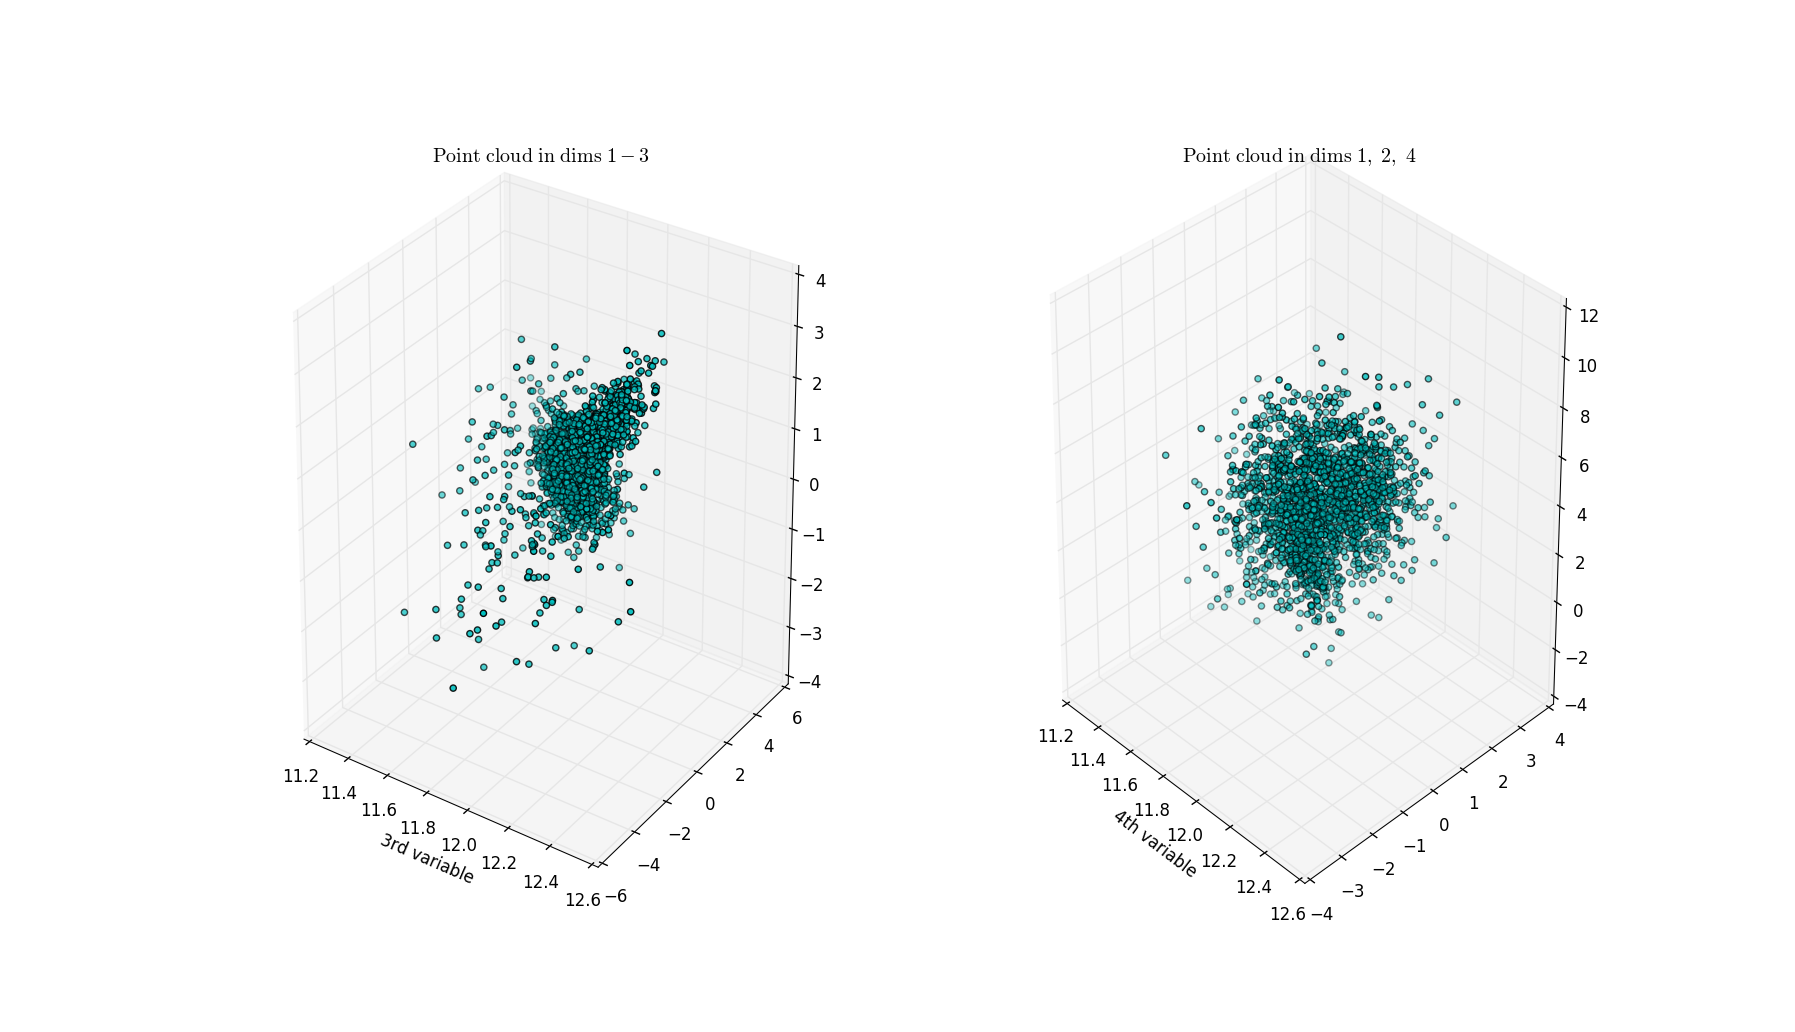
\includegraphics{../Figures/Ex3_1_scatters.png}
		\caption{Point clouds do not show significant features, other than correlation between $x_1, x_2$.}
		\label{fig:31scatters}
	\end{figure}

Maybe histograms of the single dimensions tell us a bit more:

\begin{verbatim}
        fig31 = plt.figure()
        ax1 = fig31.add_subplot(221)
        n1, bins1, patches1 = plt.hist(X[ :, 0 ], 25, normed=1, alpha=0.75)
        plt.xlabel('frequency (normed)')
        plt.ylabel('value')
        plt.title(r'$\mathrm{Histogram\ in\ dim\ 1}$')
        ax2 = fig31.add_subplot(222)
        n2, bins2, patches2 = plt.hist(X[ :, 1 ], 25, normed=1, alpha=0.75)
        plt.xlabel('frequency (normed)')
        plt.ylabel('value')
        plt.title(r'$\mathrm{Histogram\ in\ dim\ 2}$')
        ax3 = fig31.add_subplot(223)
        n3, bins3, patches3 = plt.hist(X[ :, 2 ], 25, normed=1, alpha=0.75)
        plt.xlabel('frequency (normed)')
        plt.ylabel('value')
        plt.title(r'$\mathrm{Histogram\ in\ dim\ 3}$')
        ax4 = fig31.add_subplot(224)
        n4, bins4, patches4 = plt.hist(X[ :, 3 ], 25, normed=1, alpha=0.75)
        plt.xlabel('frequency (normed)')
        plt.ylabel('value')
        plt.title(r'$\mathrm{Histogram\ in\ dim\ 4}$')
        plt.show()
\end{verbatim}

This will yield the following figures:
\begin{figure}[H]
	\centering 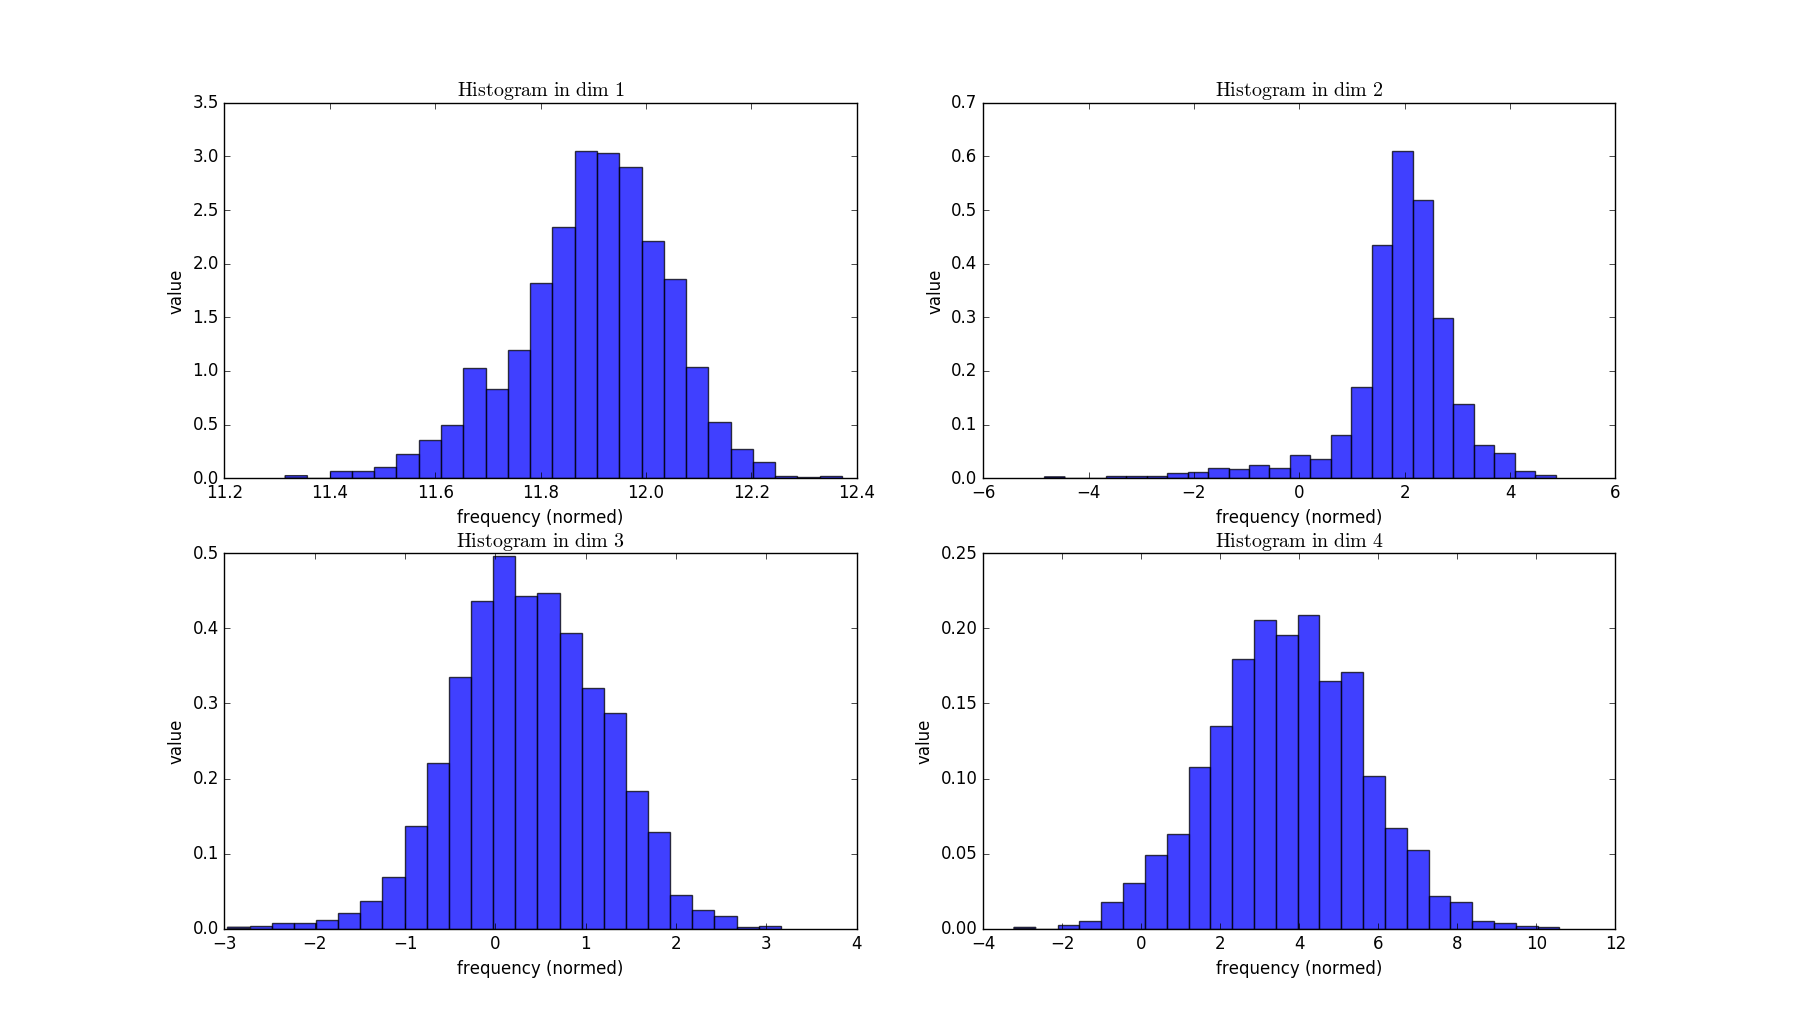
\includegraphics{../Figures/Ex3_1_hists.png}
	\caption{Histograms reveal a little more information.}
	\label{fig:3hist}
\end{figure}

Firstly, we notice that the distributions across dimensions 1 and 2 are both left-skewed. 
This does not imply a correlation, but it could be the one, we saw in the first graph.

Secondly, dimension 1 shows a little bump on the left side of the mean. This could be a mini-cluster.

\subsection{Setting up the EM-algorithm}\label{ex:3.2}
This is a pure coding exercise. All the requested features will become obvious in the next parts. The code of the EM-class is attached in the Appendix. I will only copy the relevant parts or parts from the executable script \texttt{Ex3.py} here.
The EM-class is contained in \texttt{mixture\_models.py}. It was originally based on the Gaussian mixture models from the scipy-package, but completely rewritten for this exercise and exercise 4.
For convenience and readability, the general structure and some method names remain similar.
Formulas implemented from CB06 are marked with the respective number.
To make the review easier, I will point to where the specific requested features can be found in the code.
\begin{itemize}
\item Initialisation variable setup, i.e. means, weights and covariances: 
\begin{verbatim}
        n_iterations = 100
        K = 2
        # initialisation
        init_means = np.repeat(np.mean(X, axis=0), K,
		        axis=0).reshape(K, D)
        init_means += np.random.random_sample((K, D)) * 2.0 - 1.0
        init_weights = np.ones(K, dtype=float) / K
        init_covars = np.zeros((K, D, D))
        for k in np.arange(K):
            # the initialisation cannot lead to singularity.
            Sigma_k = np.random.random_sample(D) * 4.0 + 2.0
            init_covars[ k, :, : ] = np.diag(Sigma_k)
        init_covars = init_covars[ :, :, : ]
\end{verbatim}
\item After the initialisation of the class instance, the number of iterations of the EM-steps are dynamically increased until reaching 100:
\begin{verbatim}
        loglikelihoods = np.zeros(n_iterations)
        criterions = np.zeros(n_iterations)
        convergence_print = False
        for i in np.arange(1, n_iterations):
            gmm = mixture_models.MixtureModel(
                    n_components=K,
                    means_init=init_means,
                    weights_init=init_weights,
                    covars_init=init_covars,
                    random_state=np.random.seed(1),
                    n_iter=i)
            gmm = gmm.fit(X)
            if gmm.converged_ and not convergence_print:
                print('converged at step {0}'.format(i))
                convergence_print = True
            loglikelihoods[ i ] = np.sum(gmm.score_samples(X)[ 0 ])
            criterions[ i ] = gmm.bic(X)

        # The final data labels:
        labels = gmm.score_samples(X)[ 1 ].argmax(axis=1)
\end{verbatim}
This already includes an example run in the line containing \texttt{gmm = gmm.fit(X)}, which is part of subsection \ref{ex:3.3}.
\item The plots are displayed here for the initial run, required in \ref{ex:3.3}.
\end{itemize}

We will get the following figures:
\begin{figure}[H]
	\centering 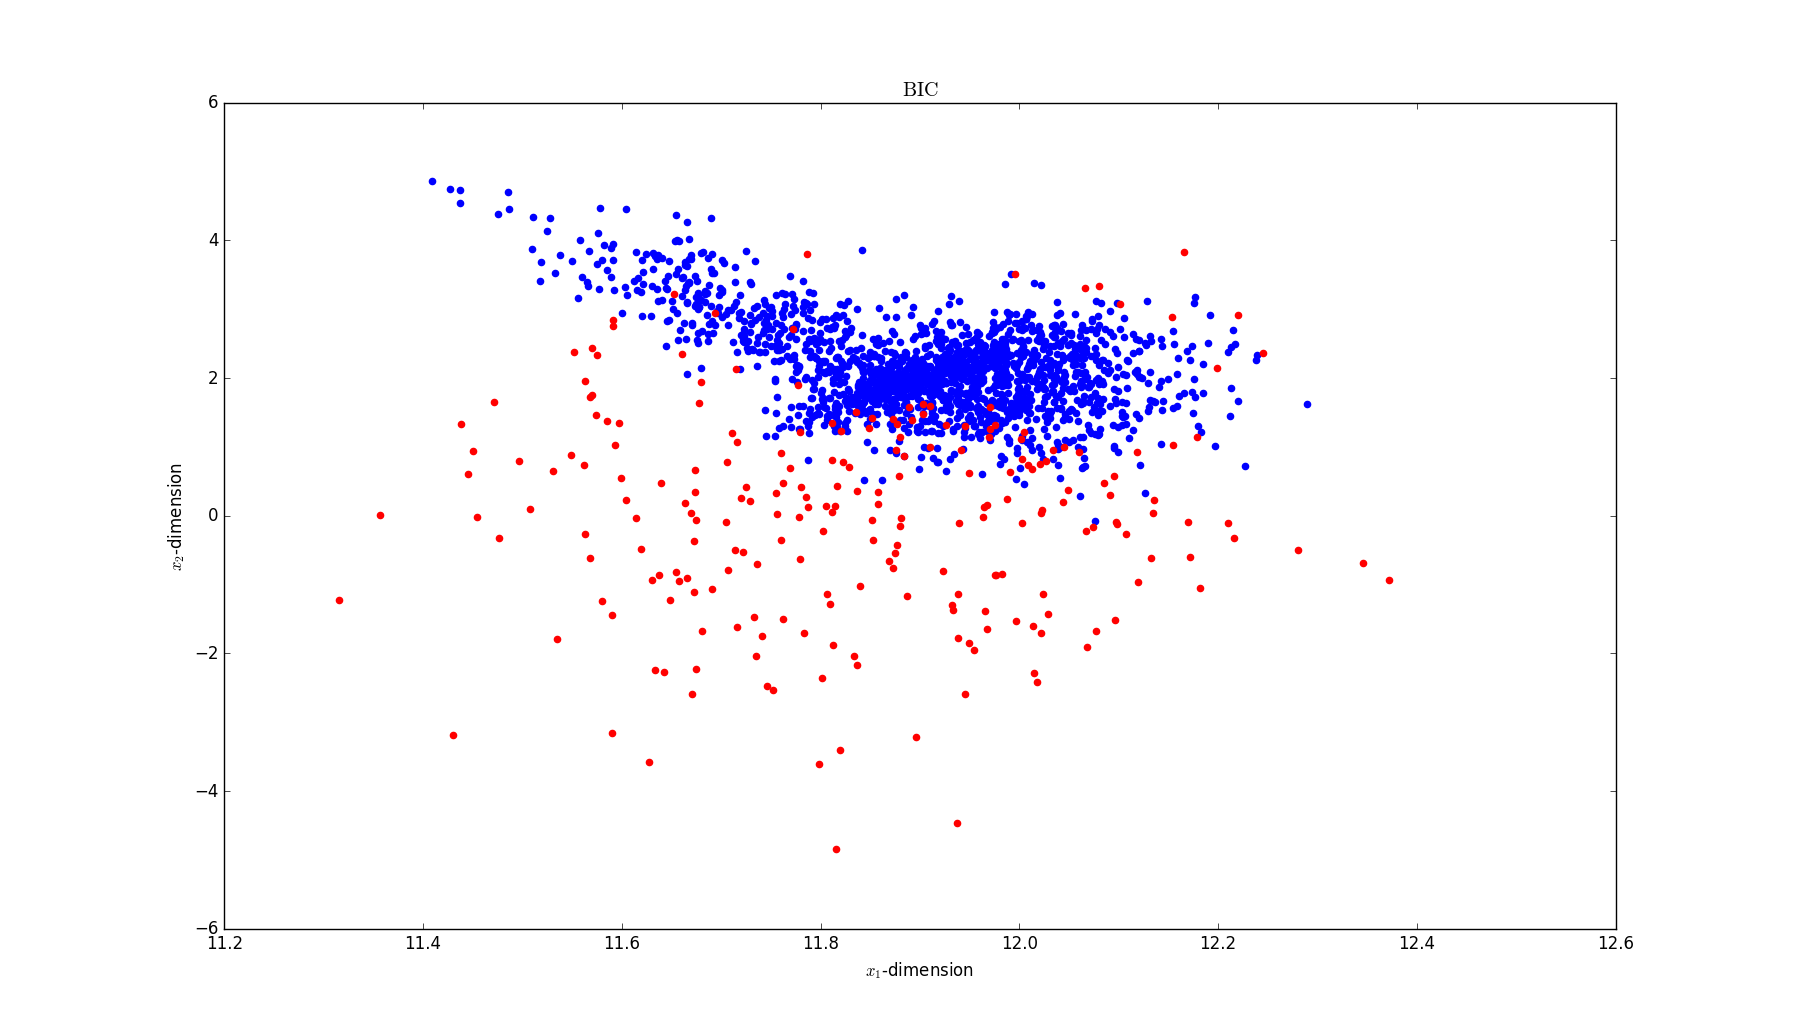
\includegraphics{../Figures/Ex3_2_scatters.png}
	\caption{It is obvious that one cluster is significantly bigger than the other. This may either be due to the 1-in-5 rumors or an unfortunate RNG initialisation. As it is unclear which cluster is which, there are no labels designated.}
	\label{fig:32scatter}
\end{figure}

Now have a look at the course of the classification procedure:
We will get the following figures:
\begin{figure}[H]
	\centering 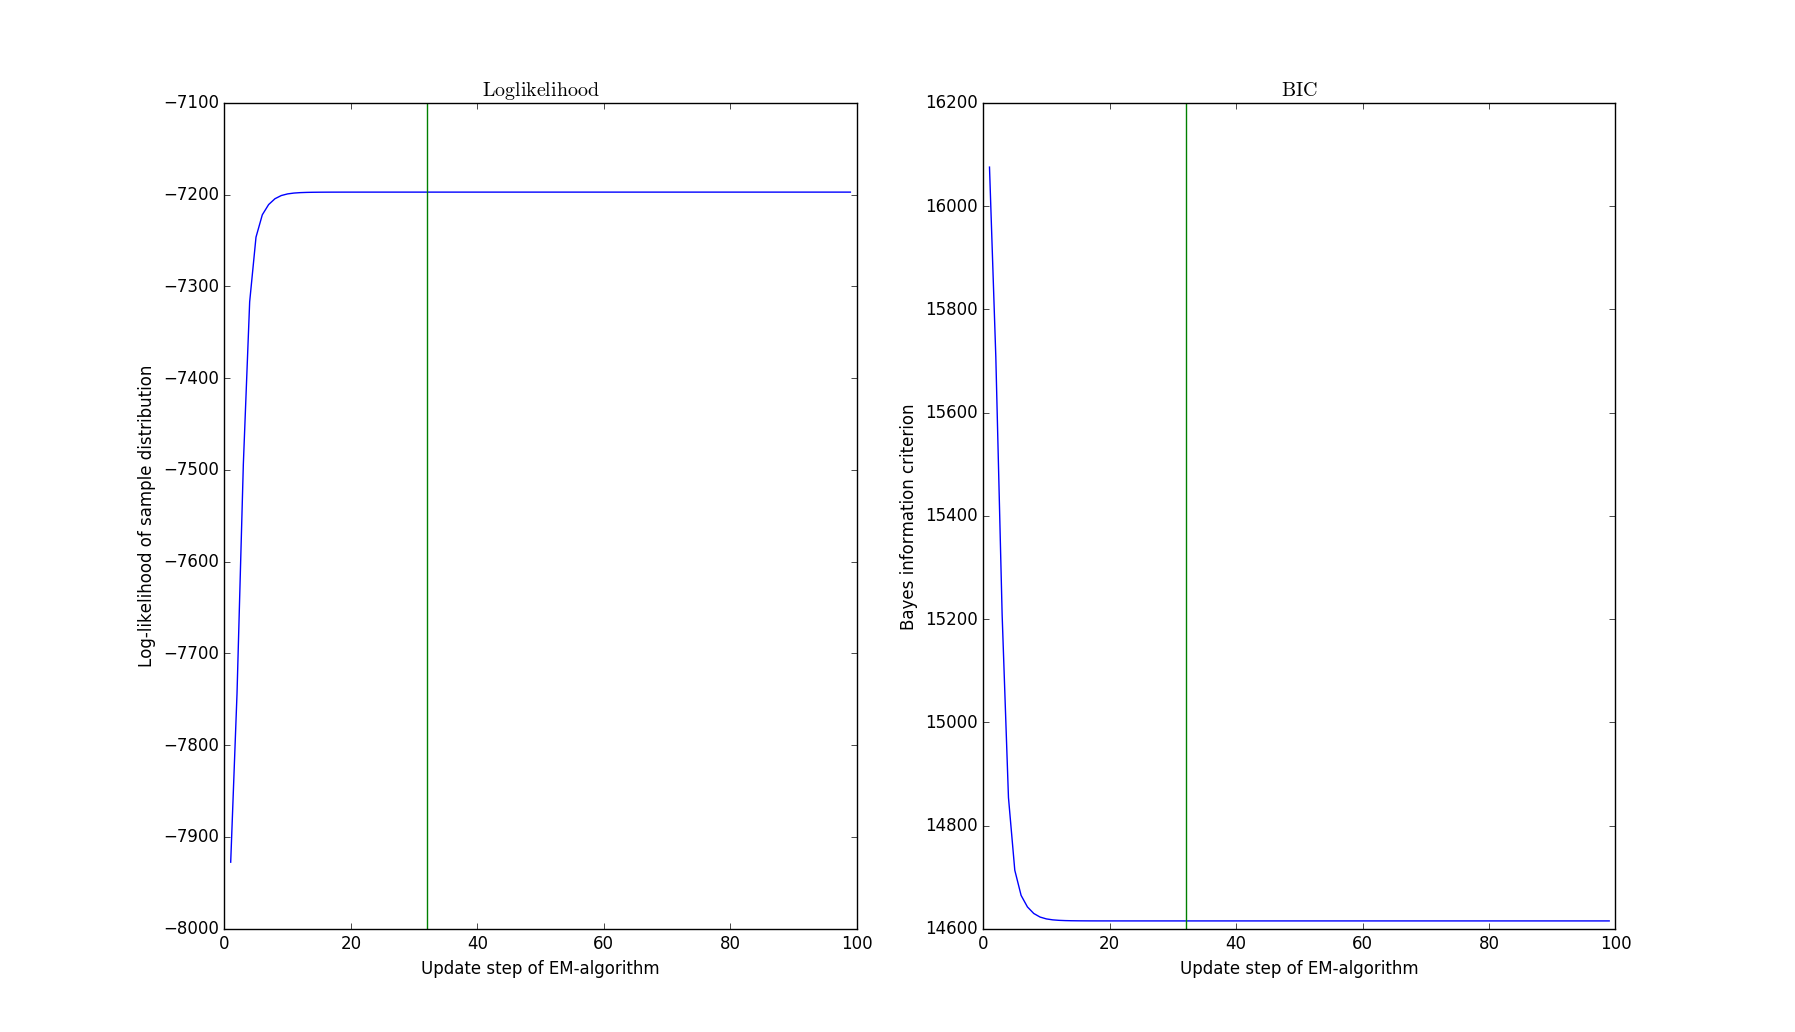
\includegraphics{../Figures/Ex3_2_llh.png}
	\caption{Depicted are the loglikelihood (left) and (due to its popularity for simple model selection) the Bayes information criterion (BIC, right). Obviously, we have a quick, close to exponential convergence. The EM-algorithm converges at step 32, marked in green, with an change in loglikelihood smaller than $10^{-8}$.}
	\label{fig:32llh}
\end{figure}

\subsection{Fitting Gaussian mixture models with EM}\label{ex:3.3}
The $K=2$-case has already been described above (see figure \ref{fig:32llh}). 

\begin{figure}[H]
	\centering 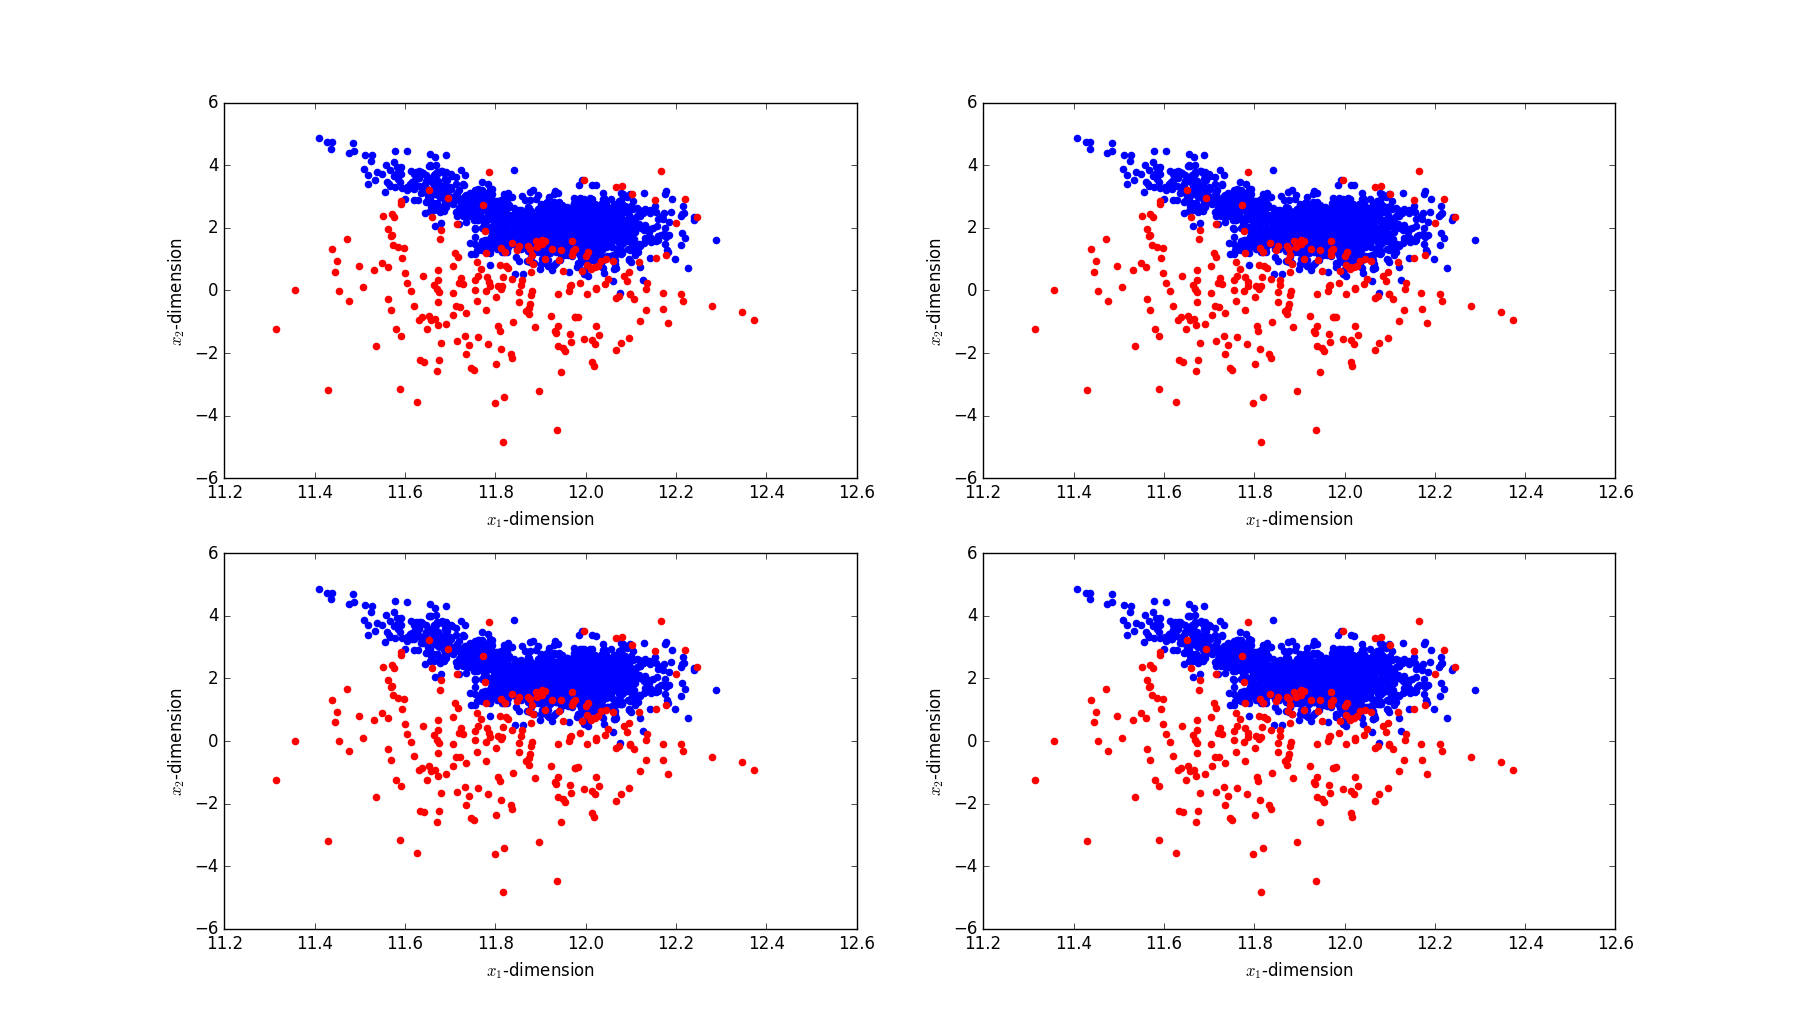
\includegraphics{../Figures/Ex3_3_scatters.png}
	\caption{The four plots show classifications from different random starting points. The classifications are similar or identical but convergence is reached unequally fast.}
	\label{fig:33scatter}
\end{figure}

If we look at the clustering from different starting points, we can not visually differentiate (see figure \ref{fig:33scatter}), however, when looking at the BIC-curves, we can see, that the algorithm converges more or less equally quickly. In fact, all the graphs look like figure \ref{fig:32llh} when not zooming in extremely. The earliest convergence measured in 8 randomised starting points was in 19 steps, the longest took 33 steps. This is marginal, considering there is only a change $<10^{-3}$ after the 6th step. Of course, this is not yet enough to reliably infer on the distribution. 

The correlation matrix of the components averaged over the different RNG initialisations is obtained the following way:
\begin{verbatim}
        # correlation coefficients
        corrcoeffs = np.zeros((K, randomisations))
        for l in np.arange(randomisations):
            for k in np.arange(K):
                submat = X[ labels2[ :, l ] == k, : ]
                corrcoeffs[ k, l ] = \
                    np.corrcoef(submat[ :, 0 ], submat[ :, 1 ])[ 0, 1 ]
        corrcoeffs = np.mean(corrcoeffs, axis=1)
        print(corrcoeffs)

\end{verbatim}
This gives:
\begin{align}
R^{(K=2)} = \begin{pmatrix}
-0.38041957 & -0.06159985
\end{pmatrix}
\end{align}
We can see that there is a medaite correlation between dimensions $x_1$ and $x_2$. We will thus continue and investigate further instances.

\subsection{Gaussian mixture models with 3 components}\label{ex:3.4}
If we increase $K=3$ or $K=4$ and otherwise keep the code from section \ref{ex:3.3}, we will obtain the following clustering (examples):

\begin{figure}[H]
	\centering 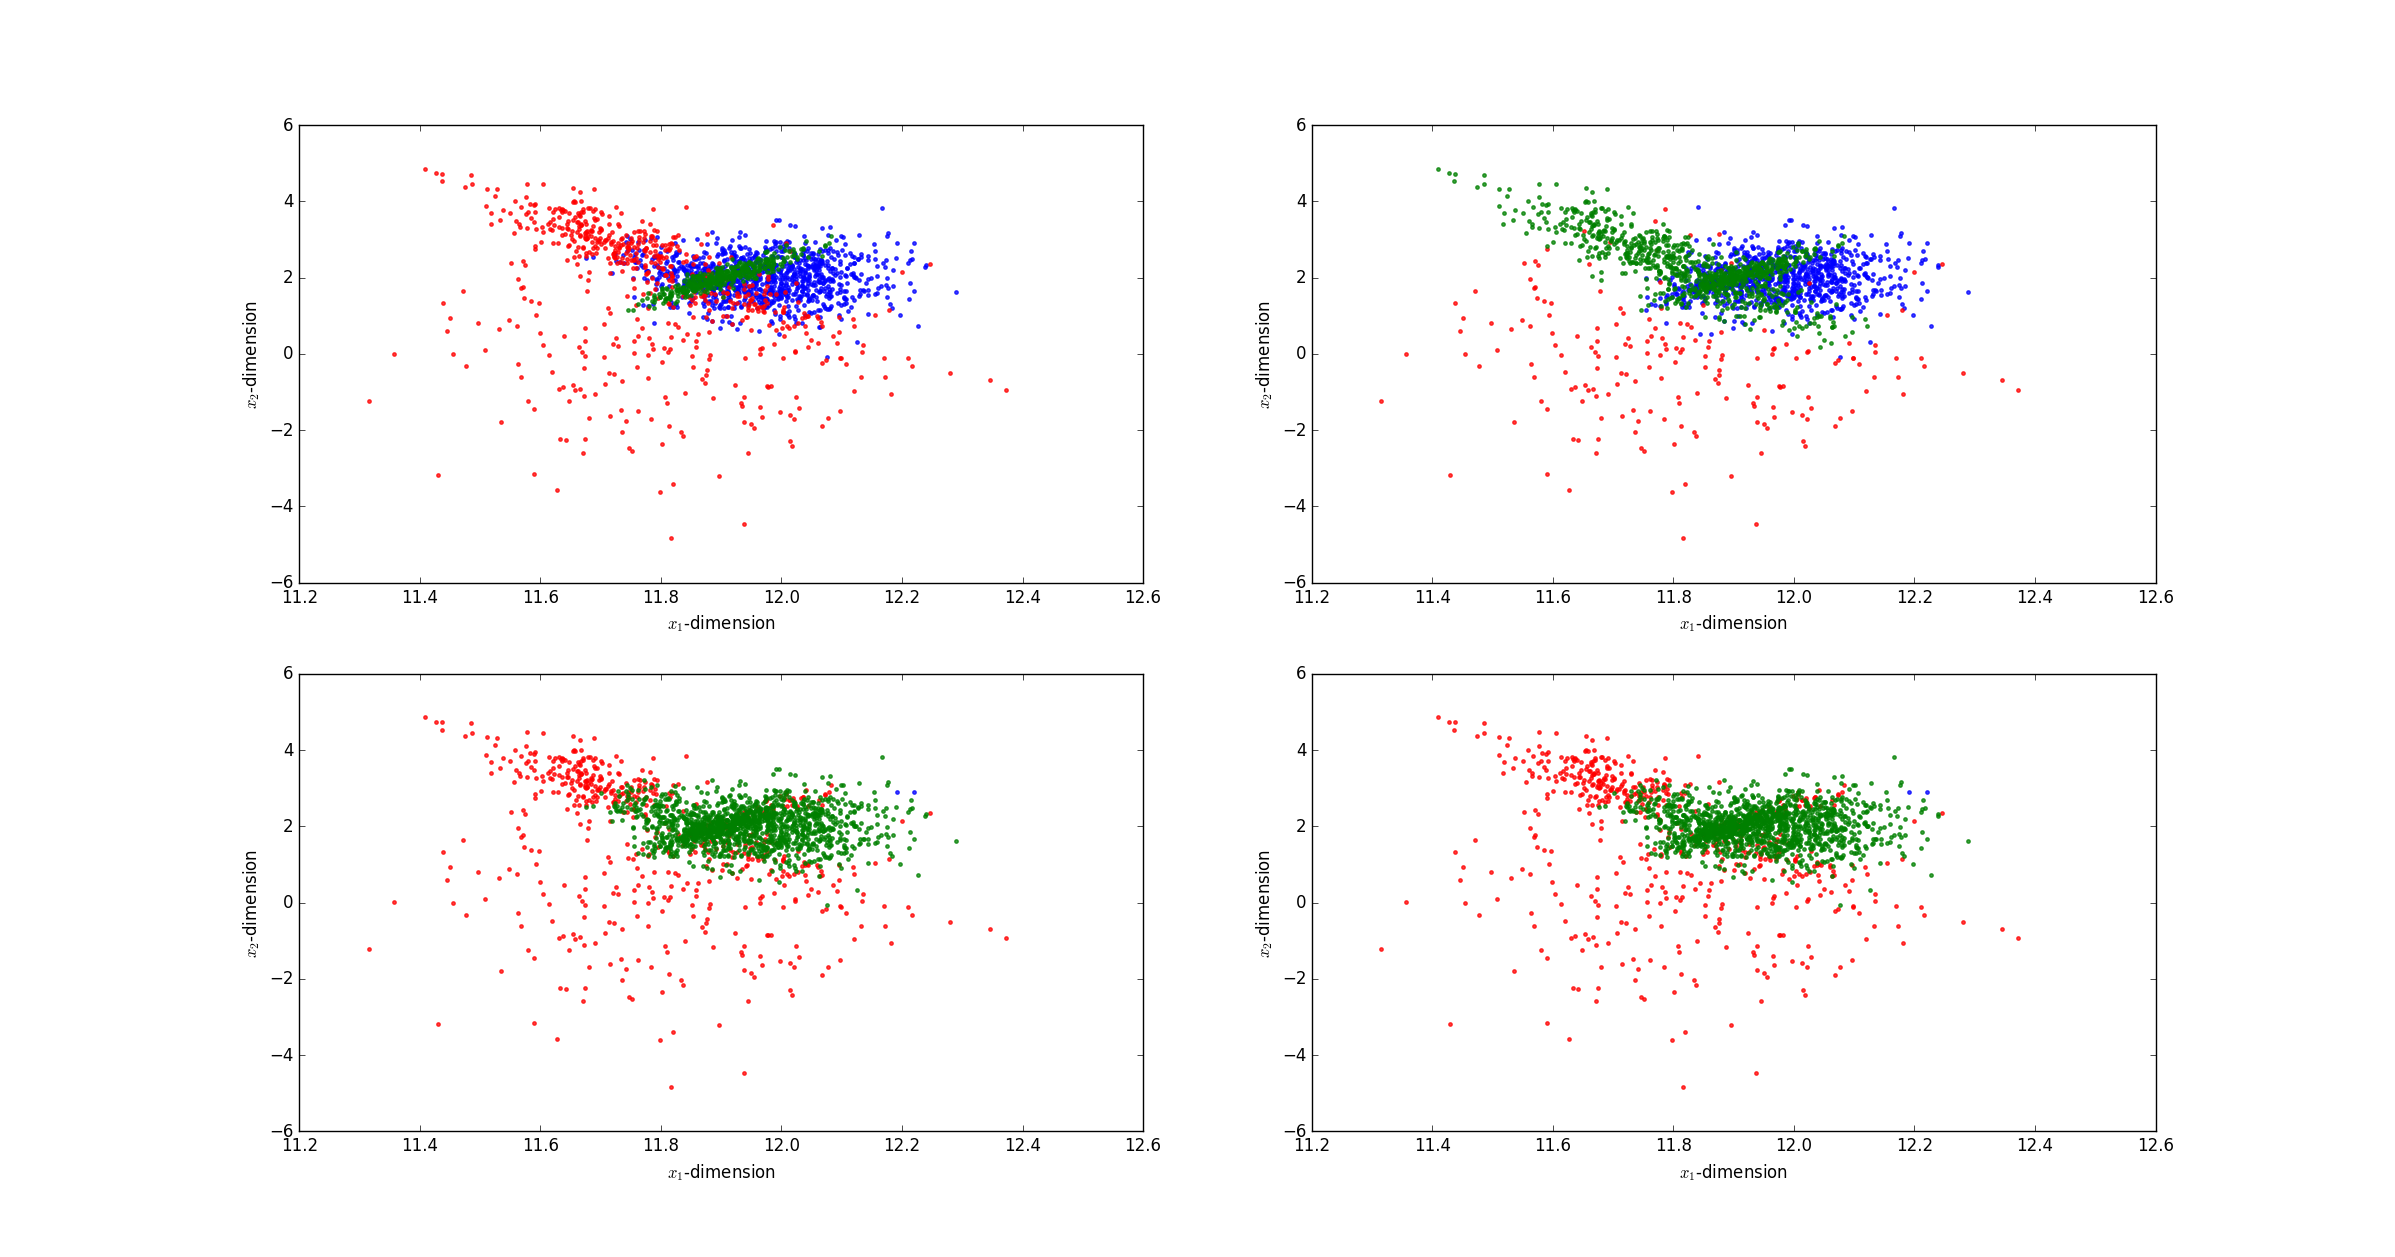
\includegraphics{../Figures/Ex3_4_scatters1.png}
	\caption{From left to right, top to bottom, the \textcolor{blue}{best}, \textcolor{yellow}{second-best}, \textcolor{red}{third-best} and \textcolor{green}{worst} classification with $K=3$ components measured by BIC, colors corresponding to curves in \ref{fig:34llh1}.}
	\label{fig:34scatter1}
\end{figure}

\begin{figure}[H]
	\centering 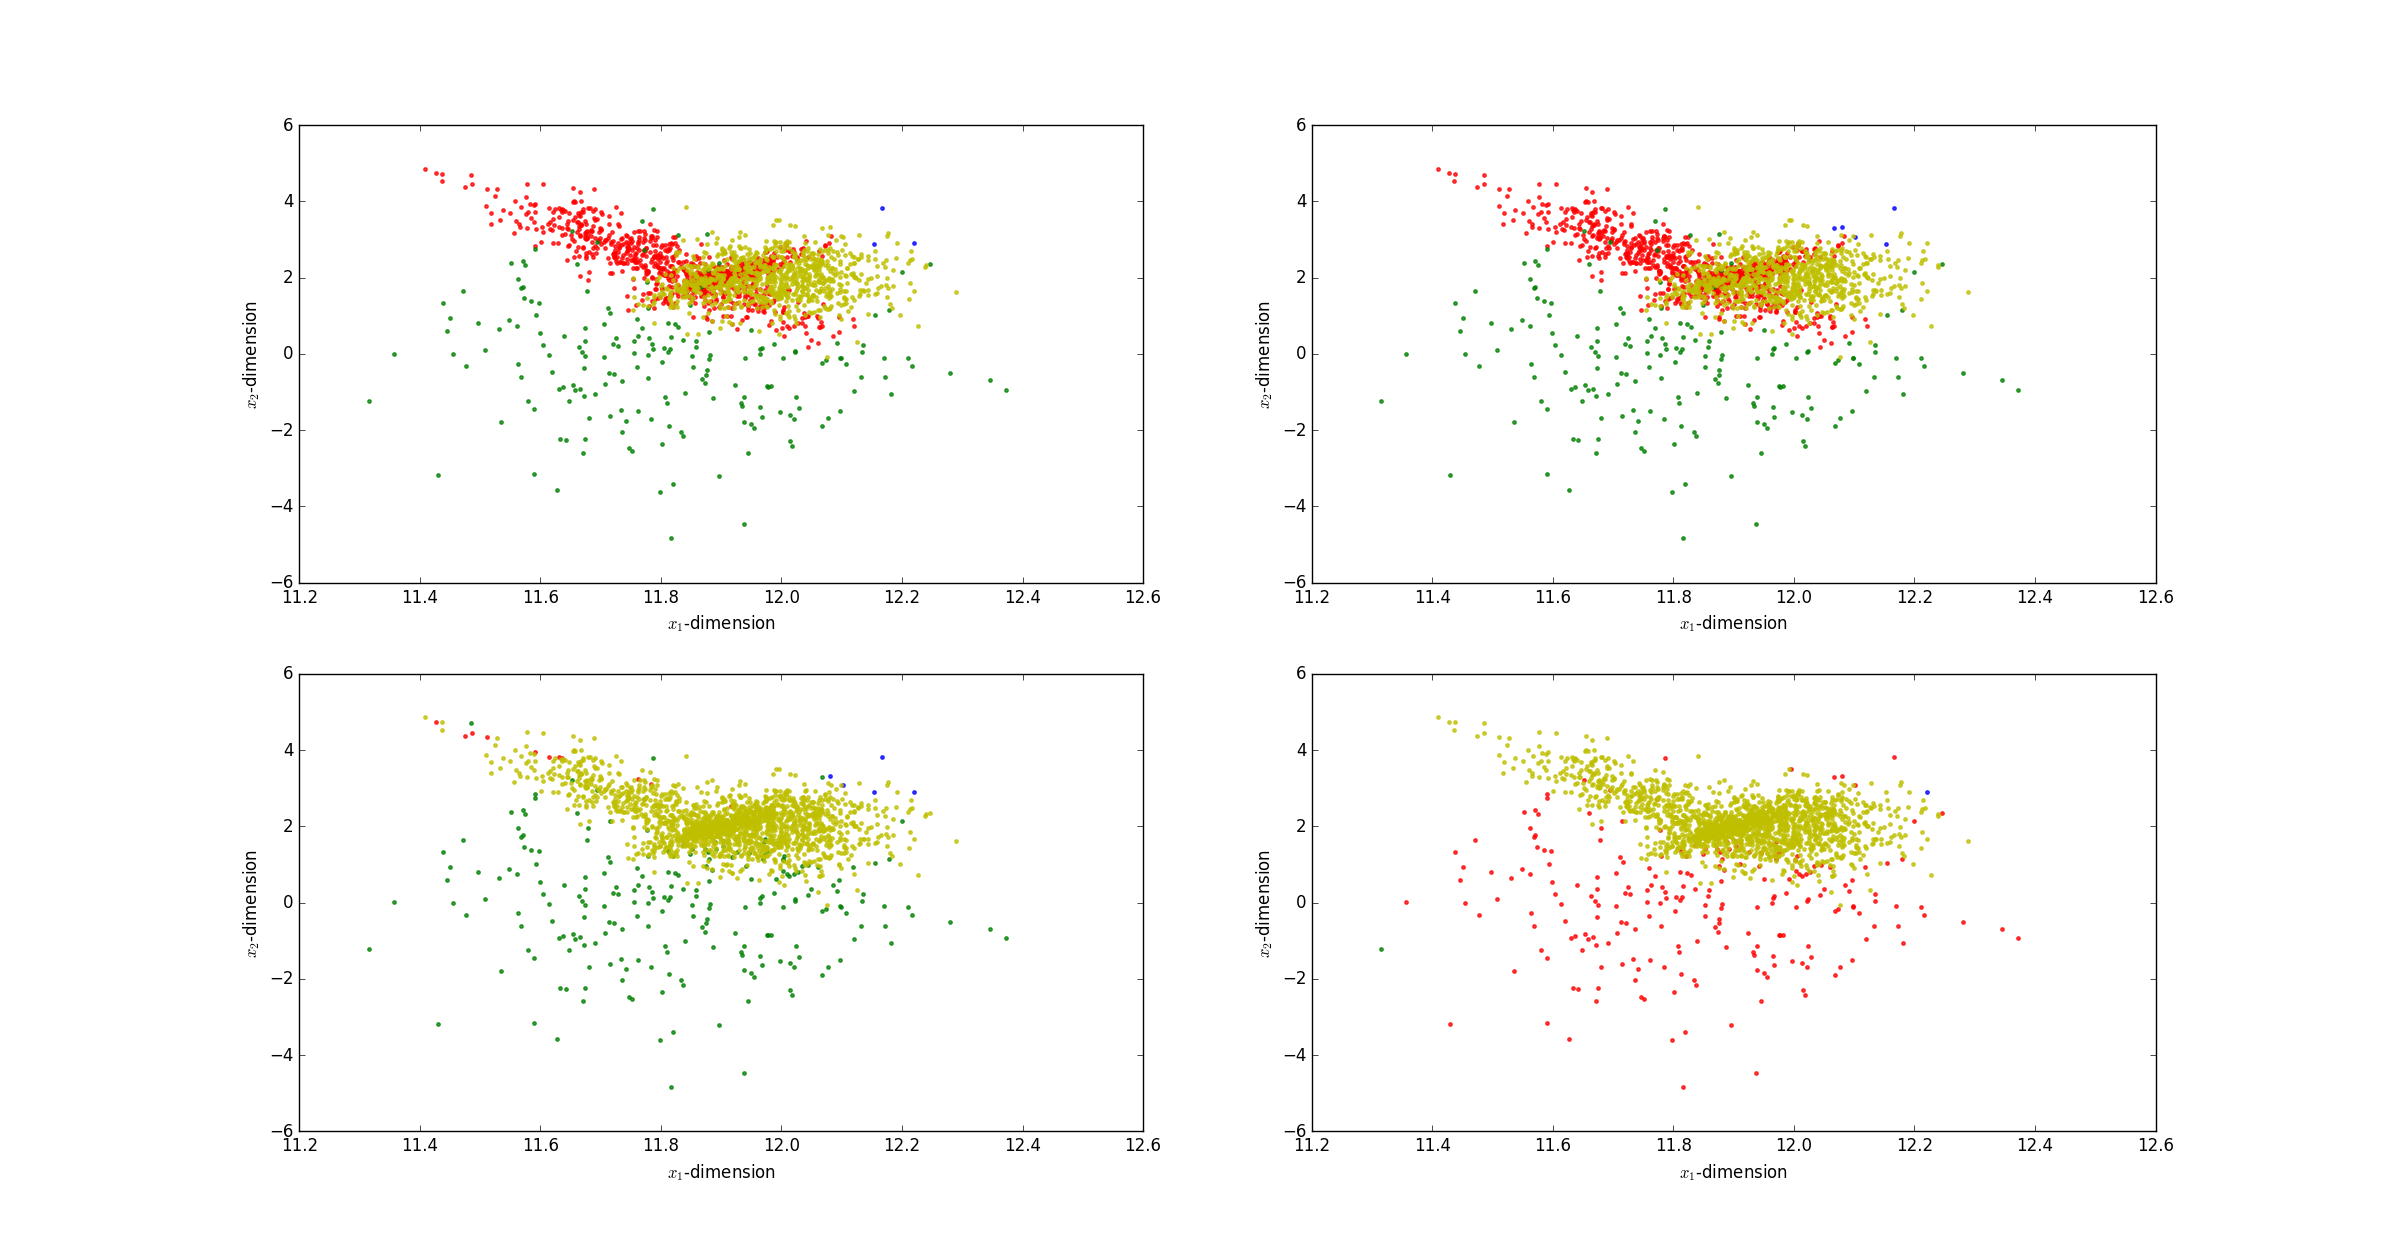
\includegraphics{../Figures/Ex3_4_scatters2.png}
	\caption{From left to right, top to bottom, the \textcolor{blue}{best}, \textcolor{green}{second-best}, \textcolor{red}{third-best} and \textcolor{yellow}{worst} classification with $K=4$ components measured by BIC, colors corresponding to curves in \ref{fig:34llh2}.}
	\label{fig:34scatter2}
\end{figure}

For the mean across eight initialisations, we get the following correlations between the first two components:
\begin{align}
R^{(K=3)} = \begin{pmatrix}
-0.4350281 & -0.29754575 & -0.0639132
\end{pmatrix}
\end{align}
and
\begin{align}
R^{(K=4)} = \begin{pmatrix}
0.30244767 & -0.59228445 & -0.20562716 & -0.03762572
\end{pmatrix}
\end{align}
We can now see that the first two variables in the first components of the $K=3$ and $K=4$ solutions show intermediate correlations and the second component in the $K=4$ solution has the strong correlation between $x_1$ and $x_2$, but the solution has a significantly higher BIC than the $K=3$ solution:

\begin{figure}[H]
	\centering 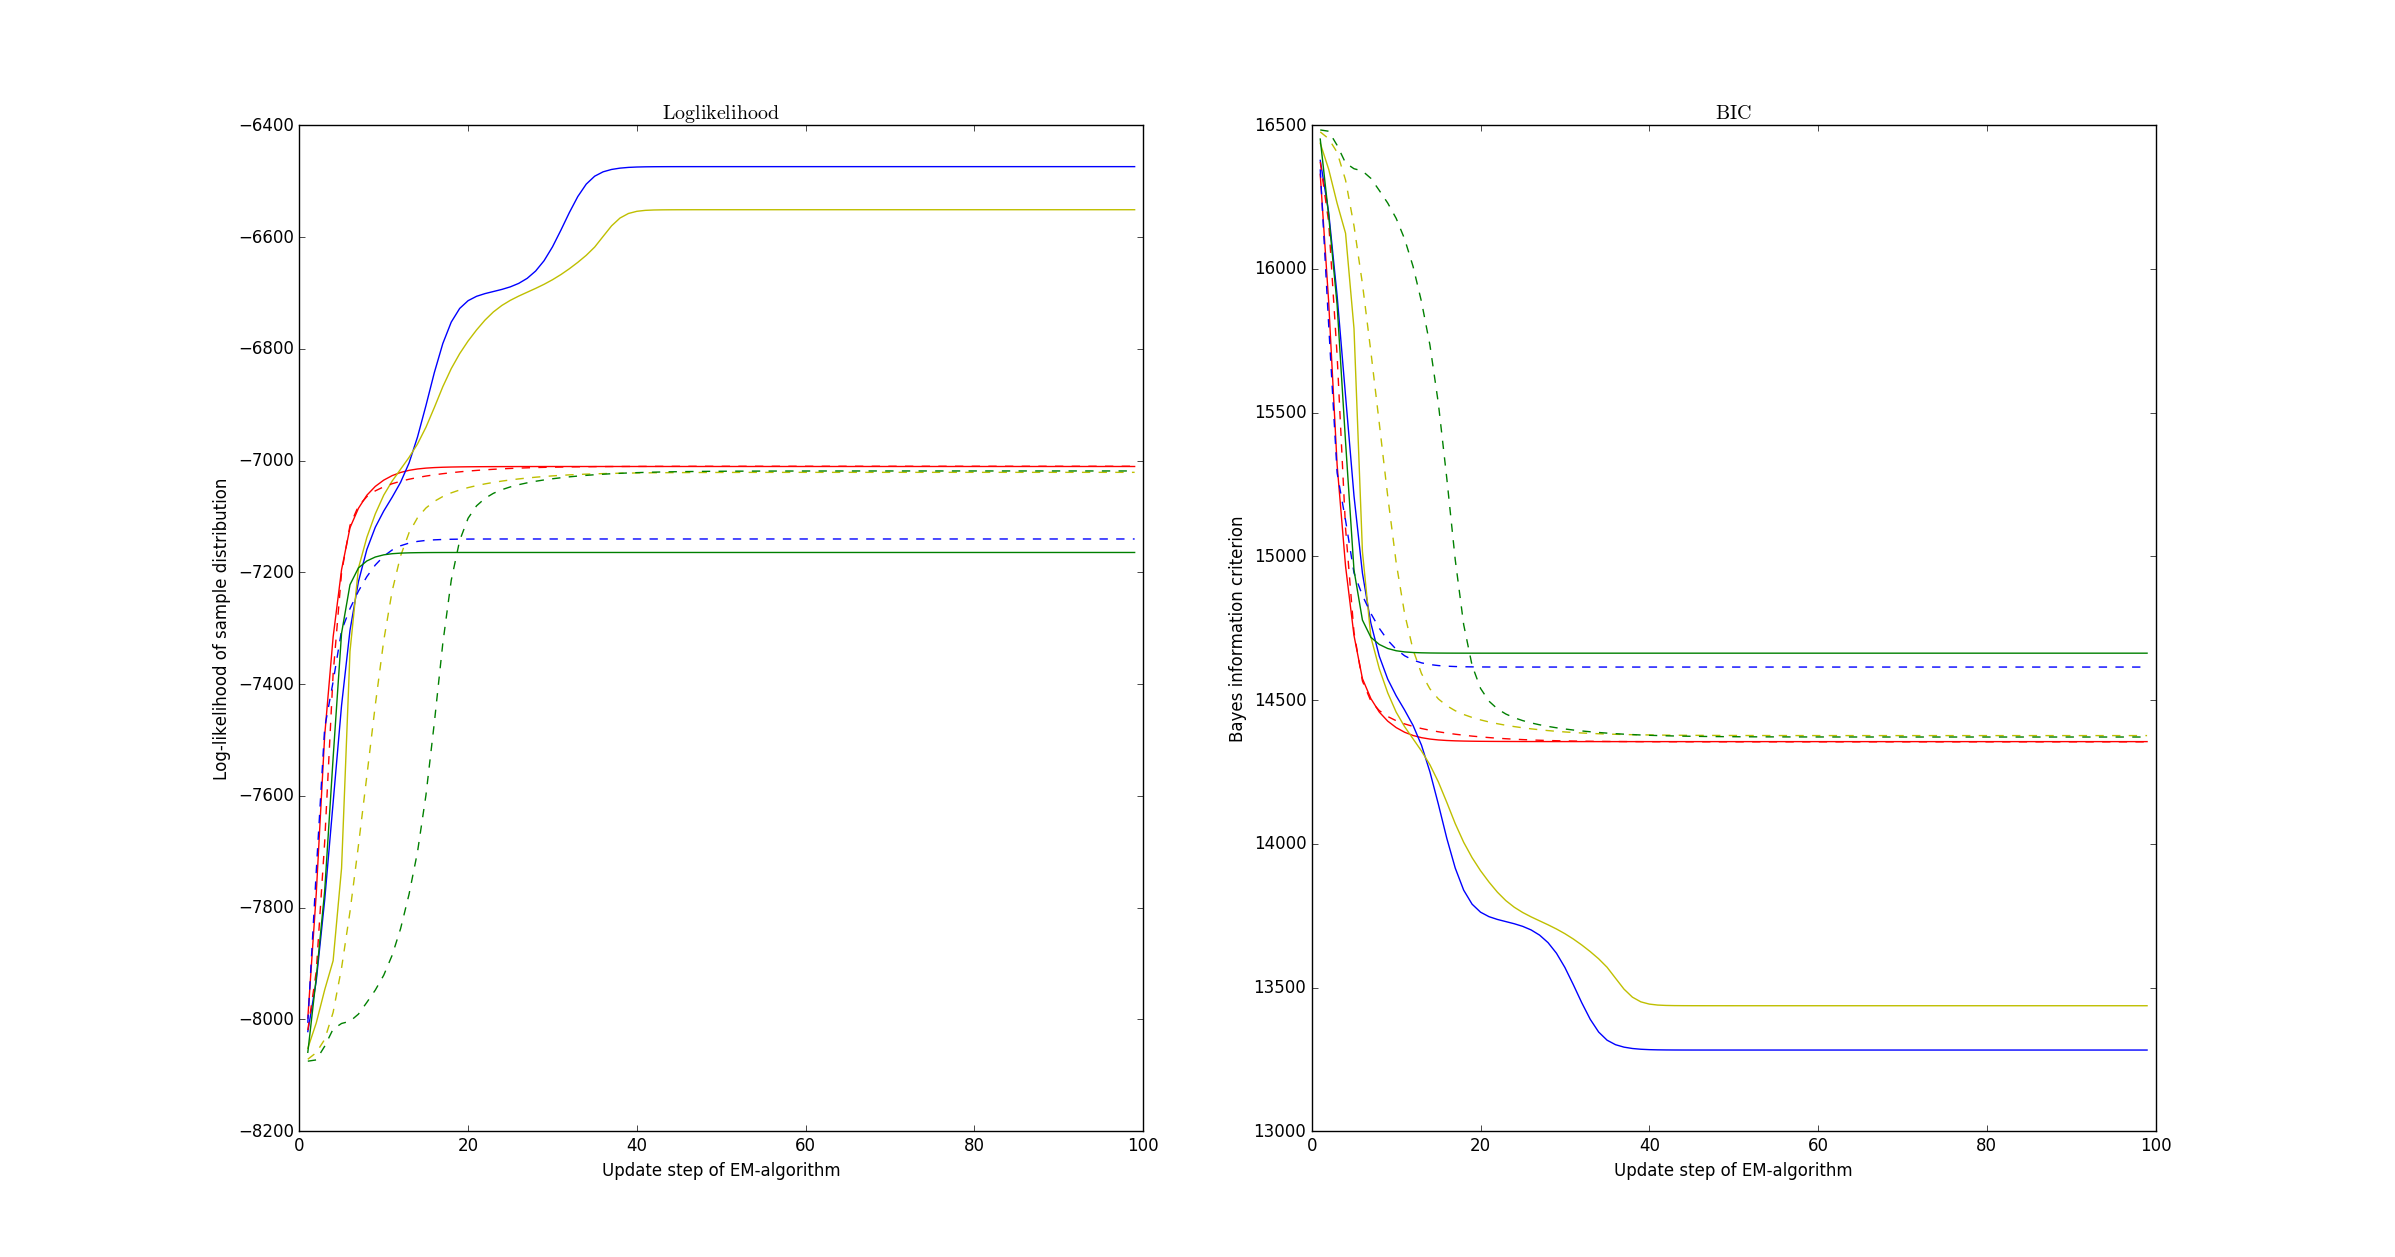
\includegraphics{../Figures/Ex3_4_llh1.png}
	\caption{Criteria for 8 random starting points for means and covariance matrices for $K=3$ clusters. The upper cluster of curves in the BIC plot apparently falls into a local minimum. The blue and yellow curves avoid this one and one additional minimum around $\mathrm{BIC}=13700$}. The classification scatter plots for the blue, yellow, red and green curves are shown in figure \ref{fig:34scatter1}.
	\label{fig:34llh1}
\end{figure}

\begin{figure}[H]
	\centering 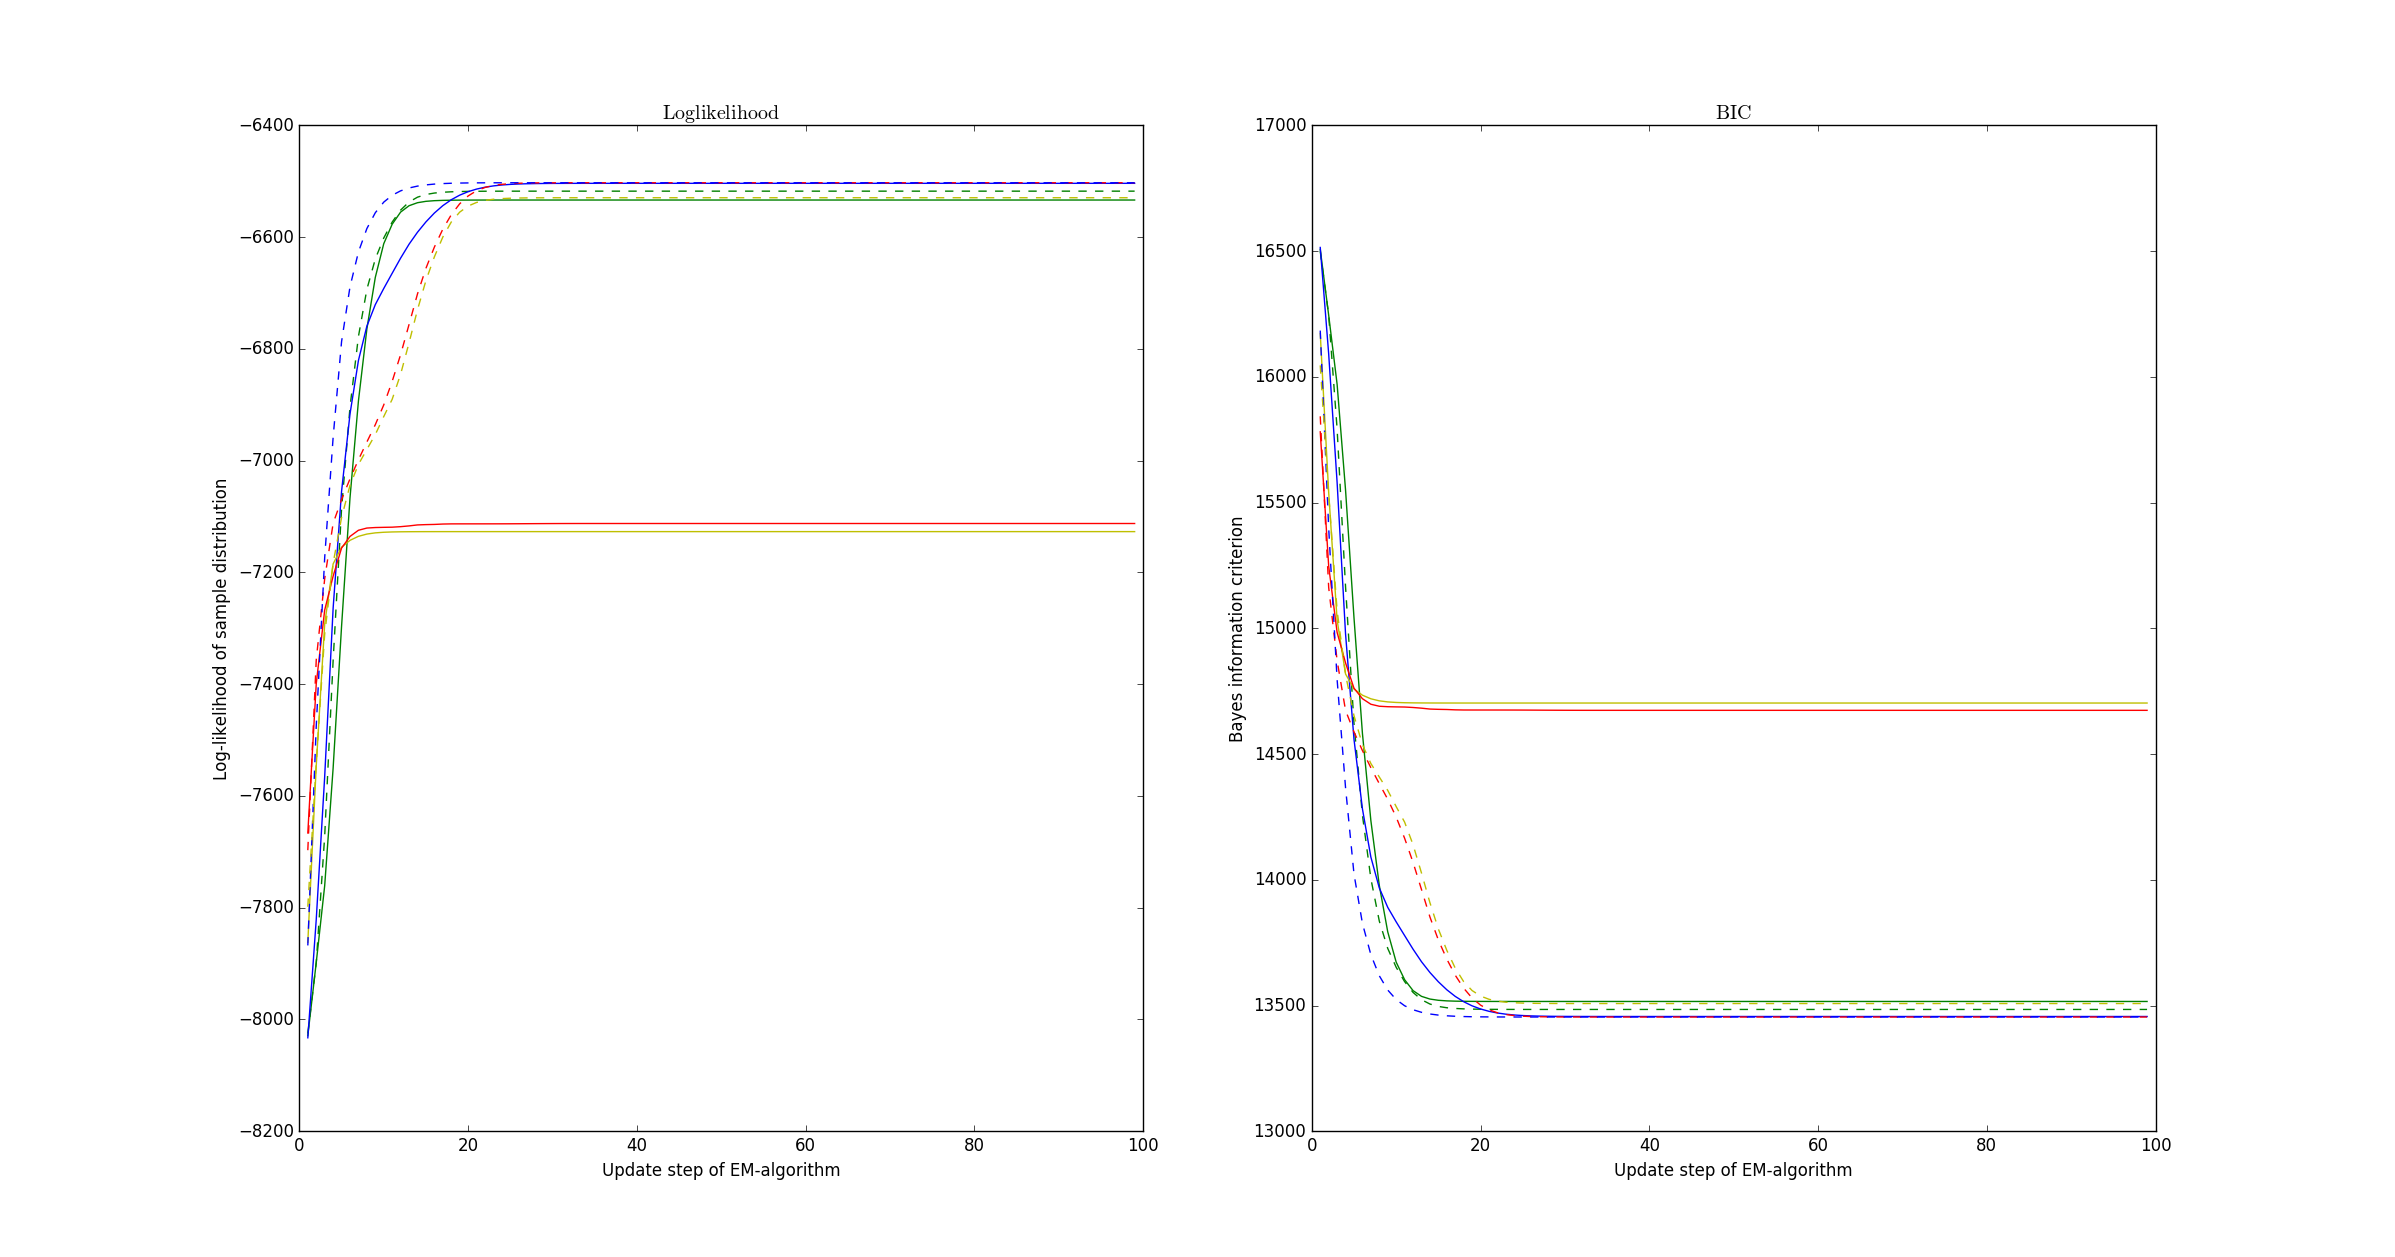
\includegraphics{../Figures/Ex3_4_llh2.png}
	\caption{Criteria for 8 random starting points for means and covariance matrices for $K=3$ clusters. There are again local minima, which are avoided by some instances, but the BIC for the optimal solution is higher than the one of case blue in figure \ref{fig:34llh1}, so the 3-Cluster solution is to be preferred.}
	\label{fig:34llh2}
\end{figure}

Our favourite candidates so far are the blue and yellow instances from the $K=3$ approach. The specific  correlations for these cases are
\begin{align}
R_{12}^{\mathrm{blue}} = \begin{pmatrix}
-0.07132327 & -0.40488436 &  0.91446507
\end{pmatrix}
\end{align}
and \begin{align}
R_{12}^{\mathrm{yellow}} = 
\begin{pmatrix}
0.12459622, -0.12769156, -0.72187397
\end{pmatrix}
\end{align}
This fits nicely, as we can then say that the best solution is blue with the third component having the high correlation between variables $x_1$ and $x_2$ and thus containing the samples with substance $X$. The number of points mapped to this cluster is \texttt{np.sum(labels3 == 2)} $ = 406$, so 1 in 5 is indeed appropriate! Cluster 1 has 974 cases (which we assume to be okay) and cluster to contains 620 cases, which are undecided.

\subsection{Prediction for new samples}
Now, let's do something dangerous, because you should never infer from the statistics on the single case...
\begin{verbatim}
        # Here are our possible culprits:
        newsamples = np.array([ [ 11.85, 2.2, 0.5, 4.0 ],
                                [ 11.95, 3.1, 0.0, 1.0 ],
                                [ 12.00, 2.5, 0.0, 2.0 ],
                                [ 12.00, 3.0, 1.0, 6.3 ] ])
        alpha = gmm2.predict_proba(newsamples)
\end{verbatim}

We get: 
\begin{align}
	\alpha = 
	\begin{pmatrix}
	\mathbf{ .25357808e-01} &   7.43299250e-02 &  3.12267174e-04 \\
	2.67197658e-07 &   \mathbf{9.99999715e-01} &  1.75890986e-08 \\
	8.94732884e-05 &   7.57923921e-03 &  \mathbf{9.92331288e-01} \\
	\mathbf{9.76578326e-01} &   2.34216745e-02 &  5.81372639e-13
	\end{pmatrix}
\end{align}

From the boldfaced numbers, we deduce that sample C is the sample generated after consumption of substance $X$ and sample $B$ has been tampered with.

\newpage
\begin{verbatim}
"""
This is a default script that should be adapted to the respective purpose.
"""

import numpy as np
from scipy import linalg
import os
from mpl_toolkits.mplot3d import Axes3D
import matplotlib.pyplot as plt
import numbers
import matplotlib as mpl
import matplotlib.cm as cmx
import mixture_models
from itertools import combinations

cm = mpl.colors.ListedColormap('YlGnBu')
seashore = cm = plt.get_cmap('YlGnBu')
scalarMap = cmx.ScalarMappable(cmap=seashore)
plt.clf()

if __name__ == '__main__':
    # let us first load the data:
    os.chdir('../Data/')
    X = np.loadtxt('a011_mixdata.txt')
    os.chdir('../Code/')
    N, D = X.shape
    # n = number of datapoints
    # D = number of features

    ex31 = False
    ex32 = False
    ex33 = False
    ex34 = False
    ex35 = True

    if ex31:
        """
        Exercise 3.1
        """
        fig = plt.figure()
        ax = fig.add_subplot(121, projection='3d')
        ax.scatter(X[ :, 0 ], X[ :, 1 ], X[ :, 2 ], c='c', marker='o',  s=6, alpha=0.75)
        ax.set_xlabel('1st variable')
        ax.set_ylabel('2nd variable')
        ax.set_zlabel('3rd variable')
        plt.title(r'$\mathrm{Point\ cloud\ in\ dims\ 1-3}$')
        ax2 = fig.add_subplot(122, projection='3d')
        ax2.scatter(X[ :, 0 ], X[ :, 2 ], X[ :, 3 ], c='c', marker='o',  s=6, alpha=0.75)
        ax2.set_xlabel('1st variable')
        ax2.set_ylabel('2th variable')
        ax2.set_zlabel('4th variable')
        plt.title(r'$\mathrm{Point\ cloud\ in\ dims\ 1,\ 2,\ 4}$')

        fig31 = plt.figure()
        ax1 = fig31.add_subplot(221)
        n1, bins1, patches1 = plt.hist(X[ :, 0 ], 25, normed=1, alpha=0.75)
        plt.xlabel('frequency (normed)')
        plt.ylabel('value')
        plt.title(r'$\mathrm{Histogram\ in\ dim\ 1}$')
        ax2 = fig31.add_subplot(222)
        n2, bins2, patches2 = plt.hist(X[ :, 1 ], 25, normed=1, alpha=0.75)
        plt.xlabel('frequency (normed)')
        plt.ylabel('value')
        plt.title(r'$\mathrm{Histogram\ in\ dim\ 2}$')
        ax3 = fig31.add_subplot(223)
        n3, bins3, patches3 = plt.hist(X[ :, 2 ], 25, normed=1, alpha=0.75)
        plt.xlabel('frequency (normed)')
        plt.ylabel('value')
        plt.title(r'$\mathrm{Histogram\ in\ dim\ 3}$')
        ax4 = fig31.add_subplot(224)
        n4, bins4, patches4 = plt.hist(X[ :, 3 ], 25, normed=1, alpha=0.75)
        plt.xlabel('frequency (normed)')
        plt.ylabel('value')
        plt.title(r'$\mathrm{Histogram\ in\ dim\ 4}$')
        plt.show()

    if ex32:
        """
        Exercise 3.2
        """
        # set up some stuff for the gaussian mixture models
        n_iterations = 100
        K = 2
        np.random.seed(1)
        # initialisation
        init_means = np.repeat(np.mean(X, axis=0), K, axis=0).reshape(K, D)
        init_means += np.random.random_sample((K, D)) * 2.0 - 1.0
        init_weights = np.ones(K, dtype=float) / K
        init_covars = np.zeros((K, D, D))
        for k in np.arange(K):
            # the initialisation cannot lead to singularity.
            Sigma_k = np.random.random_sample(D) * 4.0 + 2.0
            init_covars[ k, :, : ] = np.diag(Sigma_k)
        init_covars = init_covars[ :, :, : ]

        # Fit a Gaussian mixture with EM using five components
        loglikelihoods = np.zeros(n_iterations)
        criterions = np.zeros(n_iterations)
        convergence_print = False
        for i in np.arange(1, n_iterations):
            gmm = mixture_models.MixtureModel(
                    n_components=K,
                    means_init=init_means,
                    weights_init=init_weights,
                    covars_init=init_covars,
                    random_state=np.random.seed(1),
                    n_iter=i)
            gmm = gmm.fit(X)
            if gmm.converged_ and not convergence_print:
                print('converged at step {0}'.format(i))
                convergence_print = True
            loglikelihoods[ i ] = np.sum(gmm.score_samples(X)[ 0 ])
            criterions[ i ] = gmm.bic(X)

        # The final data labels:
        labels = gmm.score_samples(X)[ 1 ].argmax(axis=1)

        # let's plot the change in the loglikelihood over iterations
        fig321 = plt.figure()
        ax1 = fig321.add_subplot(121)
        ax1.plot(np.arange(1, n_iterations), loglikelihoods[ 1: ])
        plt.axvline(x=32, color='g')
        ax1.set_xlabel('Update step of EM-algorithm')
        ax1.set_ylabel('Log-likelihood of sample distribution')
        plt.title(r'$\mathrm{Loglikelihood}$')
        ax2 = fig321.add_subplot(122)
        ax2.plot(np.arange(1, n_iterations), criterions[ 1: ])
        plt.axvline(x=32, color='g')
        ax2.set_xlabel('Update step of EM-algorithm')
        ax2.set_ylabel('Bayes information criterion')
        plt.title(r'$\mathrm{BIC}$')

        # Now plot the requested colour-coded first two variables
        fig322 = plt.figure()
        ax3 = fig322.add_subplot(111)
        set0 = X[ labels == 0, : ]
        set1 = X[ labels == 1, : ]
        ax3.scatter(set0[ :, 0 ], set0[ :, 1 ], color='b', s=6, alpha=0.75)
        ax3.scatter(set1[ :, 0 ], set1[ :, 1 ], color='r', s=6, alpha=0.75)
        ax3.set_xlabel(r'$x_1$-dimension')
        ax3.set_ylabel(r'$x_2$-dimension')
        plt.title(r'$\mathrm{BIC}$')
        plt.show()

    if ex33:
        """
        Exercise 3.3
        """
        # The above version was a test run. Now some different initialisations:
        randomisations = 8
        n_iterations = 50
        loglikelihoods2 = np.zeros((n_iterations, randomisations))
        criterions2 = np.zeros((n_iterations, randomisations))
        labels2 = np.zeros((X.shape[ 0 ], randomisations))
        K = 2

        for j in np.arange(randomisations):
            np.random.seed(j)

            # initialisation
            init_means = np.repeat(np.mean(X, axis=0), K, axis=0).reshape(K, D)
            init_means += np.random.random_sample((K, D)) * 2.0 - 1.0
            init_weights = np.ones(K, dtype=float) / K
            init_covars = np.zeros((K, D, D))
            for k in np.arange(K):
                # the initialisation cannot lead to singularity.
                Sigma_k = np.random.random_sample(D) * 4.0 + 2.0
                init_covars[ k, :, : ] = np.diag(Sigma_k)
            init_covars = init_covars[ :, :, : ]

            # Fit a Gaussian mixture with EM using five components
            convergence_print = False
            for i in np.arange(0, n_iterations):
                # the data get quite big so we overwrite it every time
                gmm2 = mixture_models.MixtureModel(
                        n_components=K, n_iter=i,
                        means_init=init_means, weights_init=init_weights,
                        covars_init=init_covars,
                        random_state=np.random.seed(randomisations)
                )
                gmm2 = gmm2.fit(X)
                if gmm2.converged_ and not convergence_print:
                    print('converged at step {0}'.format(i))
                    convergence_print = True
                loglikelihoods2[ i, : ] = np.sum(gmm2.score_samples(X)[ 0 ])
                criterions2[ i, : ] = gmm2.bic(X)
            if not gmm2.converged_:
                print('no convergence in trial {0}'.format(j))
            # The final data labels:
            labels2[ :, j ] = gmm2.score_samples(X)[ 1 ].argmax(axis=1)

        # let's plot the change in the loglikelihood over iterations
        fig331 = plt.figure()
        ax1 = fig331.add_subplot(121)
        ax1.plot(np.arange(1, n_iterations), loglikelihoods2[ 1:, 1 ], 'r',
                 np.arange(1, n_iterations), loglikelihoods2[ 1:, 2 ], 'g',
                 np.arange(1, n_iterations), loglikelihoods2[ 1:, 3 ], 'b',
                 np.arange(1, n_iterations), loglikelihoods2[ 1:, 4 ], 'y',
                 np.arange(1, n_iterations), loglikelihoods2[ 1:, 5 ], 'r--',
                 np.arange(1, n_iterations), loglikelihoods2[ 1:, 6 ], 'g--',
                 np.arange(1, n_iterations), loglikelihoods2[ 1:, 7 ], 'b--',
                 np.arange(1, n_iterations), loglikelihoods2[ 1:, 0 ], 'y--'
                 )
        ax1.set_xlabel('Update step of EM-algorithm')
        ax1.set_ylabel('Log-likelihood of sample distribution')
        plt.title(r'$\mathrm{Loglikelihood}$')
        ax2 = fig331.add_subplot(122)
        ax2.plot(np.arange(1, n_iterations), criterions2[ 1:, 1 ], 'r',
                 np.arange(1, n_iterations), criterions2[ 1:, 2 ], 'g',
                 np.arange(1, n_iterations), criterions2[ 1:, 3 ], 'b',
                 np.arange(1, n_iterations), criterions2[ 1:, 4 ], 'y',
                 np.arange(1, n_iterations), criterions2[ 1:, 5 ], 'r--',
                 np.arange(1, n_iterations), criterions2[ 1:, 6 ], 'g--',
                 np.arange(1, n_iterations), criterions2[ 1:, 7 ], 'b--',
                 np.arange(1, n_iterations), criterions2[ 1:, 0 ], 'y--'
                 )
        ax2.set_xlabel('Update step of EM-algorithm')
        ax2.set_ylabel('Bayes information criterion')
        plt.title(r'$\mathrm{BIC}$')

        # scatter plots
        fig332 = plt.figure()
        ax0 = fig332.add_subplot(221)
        set0 = X[ labels2[ :, 0 ] == 0, : ]
        set1 = X[ labels2[ :, 0 ] == 1, : ]
        ax0.scatter(set0[ :, 0 ], set0[ :, 1 ], color='b', s=6, alpha=0.75)
        ax0.scatter(set1[ :, 0 ], set1[ :, 1 ], color='r', s=6, alpha=0.75)
        ax0.set_xlabel(r'$x_1$-dimension')
        ax0.set_ylabel(r'$x_2$-dimension')
        ax1 = fig332.add_subplot(222)
        set0 = X[ labels2[ :, 2 ] == 0, : ]
        set1 = X[ labels2[ :, 2 ] == 1, : ]
        ax1.scatter(set0[ :, 0 ], set0[ :, 1 ], color='b', s=6, alpha=0.75)
        ax1.scatter(set1[ :, 0 ], set1[ :, 1 ], color='r', s=6, alpha=0.75)
        ax1.set_xlabel(r'$x_1$-dimension')
        ax1.set_ylabel(r'$x_2$-dimension')
        ax2 = fig332.add_subplot(223)
        set0 = X[ labels2[ :, 4 ] == 0, : ]
        set1 = X[ labels2[ :, 4 ] == 1, : ]
        ax2.scatter(set0[ :, 0 ], set0[ :, 1 ], color='b', s=6, alpha=0.75)
        ax2.scatter(set1[ :, 0 ], set1[ :, 1 ], color='r', s=6, alpha=0.75)
        ax2.set_xlabel(r'$x_1$-dimension')
        ax2.set_ylabel(r'$x_2$-dimension')
        ax3 = fig332.add_subplot(224)
        set0 = X[ labels2[ :, 6 ] == 0, : ]
        set1 = X[ labels2[ :, 6 ] == 1, : ]
        ax3.scatter(set0[ :, 0 ], set0[ :, 1 ], color='b', s=6, alpha=0.75)
        ax3.scatter(set1[ :, 0 ], set1[ :, 1 ], color='r', s=6, alpha=0.75)
        ax3.set_xlabel(r'$x_1$-dimension')
        ax3.set_ylabel(r'$x_2$-dimension')

        # correlation coefficients
        corrcoeffs2 = np.zeros((K, randomisations))
        for l in np.arange(randomisations):
            for k in np.arange(K):
                submat = X[ labels2[ :, l ] == k, : ]
                corrcoeffs2[ k, l ] = \
                    np.corrcoef(submat[ :, 0 ], submat[ :, 1 ])[ 0, 1 ]
        corrcoeffs_mean2 = np.nanmean(corrcoeffs2, axis=1)
        print(corrcoeffs_mean2)

    if ex34:
        """
        Exercise 3.4
        """
        # We move from 2 to 3 Gaussian components
        randomisations = 8
        n_iterations = 100
        loglikelihoods3 = np.zeros((n_iterations, randomisations))
        criterions3 = np.zeros((n_iterations, randomisations))
        labels3 = np.zeros((X.shape[ 0 ], randomisations))
        K = 3
        for j in np.arange(randomisations):
            np.random.seed(j)

            # initialisation
            init_means = np.repeat(np.mean(X, axis=0), K, axis=0).reshape(K, D)
            init_means += np.random.random_sample((K, D)) * 2.0 - 1.0
            init_weights = np.ones(K, dtype=float) / K
            init_covars = np.zeros((K, D, D))
            for k in np.arange(K):
                # the initialisation cannot lead to singularity.
                Sigma_k = np.random.random_sample(D) * 4.0 + 2.0
                init_covars[ k, :, : ] = np.diag(Sigma_k)
            init_covars = init_covars[ :, :, : ]

            # Fit a Gaussian mixture with EM using five components
            convergence_print = False
            for i in np.arange(0, n_iterations):
                # the data get quite big so we overwrite it every time
                gmm3 = mixture_models.MixtureModel(
                        n_components=K, n_iter=i,
                        means_init=init_means, weights_init=init_weights,
                        covars_init=init_covars,
                        random_state=np.random.seed(randomisations)
                )
                gmm3 = gmm3.fit(X)
                if gmm3.converged_ and not convergence_print:
                    print('converged at step {0}'.format(i))
                    convergence_print = True
                loglikelihoods3[ i, j ] = np.sum(gmm3.score_samples(X)[ 0 ])
                criterions3[ i, j ] = gmm3.bic(X)
            if not gmm3.converged_:
                print('no convergence in trial {0}'.format(j))
            # The final data labels:
            labels3[ :, j ] = gmm3.score_samples(X)[ 1 ].argmax(axis=1)

        # correlation coefficients
        corrcoeffs3 = np.zeros((K, randomisations))
        for l in np.arange(randomisations):
            for k in np.arange(K):
                submat = X[ labels3[ :, l ] == k, : ]
                corrcoeffs3[ k, l ] = \
                    np.corrcoef(submat[ :, 0 ], submat[ :, 1 ])[ 0, 1 ]
        corrcoeffs_mean3 = np.nanmean(corrcoeffs3, axis=1)
        print(corrcoeffs_mean3)

        # plotting
        # scatter plots
        fig342 = plt.figure()
        ax0 = fig342.add_subplot(221)
        idx = 3
        set0 = X[ labels3[ :, idx ] == 0, : ]
        set1 = X[ labels3[ :, idx ] == 1, : ]
        set2 = X[ labels3[ :, idx ] == 2, : ]
        ax0.scatter(set0[ :, 0 ], set0[ :, 1 ], color='b', s=6, alpha=0.75)
        ax0.scatter(set1[ :, 0 ], set1[ :, 1 ], color='r', s=6, alpha=0.75)
        ax0.scatter(set2[ :, 0 ], set2[ :, 1 ], color='g', s=6, alpha=0.75)
        ax0.set_xlabel(r'$x_1$-dimension')
        ax0.set_ylabel(r'$x_2$-dimension')
        ax1 = fig342.add_subplot(222)
        idx = 4
        set0 = X[ labels3[ :, idx ] == 0, : ]
        set1 = X[ labels3[ :, idx ] == 1, : ]
        set2 = X[ labels3[ :, idx ] == 2, : ]
        ax1.scatter(set0[ :, 0 ], set0[ :, 1 ], color='b', s=6, alpha=0.75)
        ax1.scatter(set1[ :, 0 ], set1[ :, 1 ], color='r', s=6, alpha=0.75)
        ax1.scatter(set2[ :, 0 ], set2[ :, 1 ], color='g', s=6, alpha=0.75)
        ax1.set_xlabel(r'$x_1$-dimension')
        ax1.set_ylabel(r'$x_2$-dimension')
        ax2 = fig342.add_subplot(223)
        idx = 1
        set0 = X[ labels3[ :, idx ] == 0, : ]
        set1 = X[ labels3[ :, idx ] == 1, : ]
        set2 = X[ labels3[ :, idx ] == 2, : ]
        ax2.scatter(set0[ :, 0 ], set0[ :, 1 ], color='b', s=6, alpha=0.75)
        ax2.scatter(set1[ :, 0 ], set1[ :, 1 ], color='r', s=6, alpha=0.75)
        ax2.scatter(set2[ :, 0 ], set2[ :, 1 ], color='g', s=6, alpha=0.75)
        ax2.set_xlabel(r'$x_1$-dimension')
        ax2.set_ylabel(r'$x_2$-dimension')
        ax3 = fig342.add_subplot(224)
        idc = 0
        set0 = X[ labels3[ :, idx ] == 0, : ]
        set1 = X[ labels3[ :, idx ] == 1, : ]
        set2 = X[ labels3[ :, idx ] == 2, : ]
        ax3.scatter(set0[ :, 0 ], set0[ :, 1 ], color='b', s=6, alpha=0.75)
        ax3.scatter(set1[ :, 0 ], set1[ :, 1 ], color='r', s=6, alpha=0.75)
        ax3.scatter(set2[ :, 0 ], set2[ :, 1 ], color='g', s=6, alpha=0.75)
        ax3.set_xlabel(r'$x_1$-dimension')
        ax3.set_ylabel(r'$x_2$-dimension')

        fig341 = plt.figure()
        ax1 = fig341.add_subplot(121)
        ax1.plot(np.arange(1, n_iterations), loglikelihoods3[ 1:, 1 ], 'r',
                 np.arange(1, n_iterations), loglikelihoods3[ 1:, 2 ], 'y--',
                 np.arange(1, n_iterations), loglikelihoods3[ 1:, 3 ], 'b',
                 np.arange(1, n_iterations), loglikelihoods3[ 1:, 4 ], 'y',
                 np.arange(1, n_iterations), loglikelihoods3[ 1:, 5 ], 'r--',
                 np.arange(1, n_iterations), loglikelihoods3[ 1:, 6 ], 'g--',
                 np.arange(1, n_iterations), loglikelihoods3[ 1:, 7 ], 'b--',
                 np.arange(1, n_iterations), loglikelihoods3[ 1:, 0 ], 'g'
                 )
        ax1.set_xlabel('Update step of EM-algorithm')
        ax1.set_ylabel('Log-likelihood of sample distribution')
        plt.title(r'$\mathrm{Loglikelihood}$')
        ax2 = fig341.add_subplot(122)
        ax2.plot(np.arange(1, n_iterations), criterions3[ 1:, 1 ], 'r',
                 np.arange(1, n_iterations), criterions3[ 1:, 2 ], 'y--',
                 np.arange(1, n_iterations), criterions3[ 1:, 3 ], 'b',
                 np.arange(1, n_iterations), criterions3[ 1:, 4 ], 'y',
                 np.arange(1, n_iterations), criterions3[ 1:, 5 ], 'r--',
                 np.arange(1, n_iterations), criterions3[ 1:, 6 ], 'g--',
                 np.arange(1, n_iterations), criterions3[ 1:, 7 ], 'b--',
                 np.arange(1, n_iterations), criterions3[ 1:, 0 ], 'g'
                 )
        ax2.set_xlabel('Update step of EM-algorithm')
        ax2.set_ylabel('Bayes information criterion')
        plt.title(r'$\mathrm{BIC}$')

        # We move from 3 to 4 Gaussian components
        randomisations = 8
        n_iterations = 100
        loglikelihoods4 = np.zeros((n_iterations, randomisations))
        criterions4 = np.zeros((n_iterations, randomisations))
        labels4 = np.zeros((X.shape[ 0 ], randomisations))
        K = 4
        for j in np.arange(randomisations):
            np.random.seed(j)

            # initialisation
            init_means = np.repeat(np.mean(X, axis=0), K, axis=0).reshape(K, D)
            init_means += np.random.random_sample((K, D)) * 2.0 - 1.0
            init_weights = np.ones(K, dtype=float) / K
            init_covars = np.zeros((K, D, D))
            for k in np.arange(K):
                # the initialisation cannot lead to singularity.
                Sigma_k = np.random.random_sample(D) * 4.0 + 2.0
                init_covars[ k, :, : ] = np.diag(Sigma_k)
            init_covars = init_covars[ :, :, : ]

            # Fit a Gaussian mixture with EM using five components
            convergence_print = False
            for i in np.arange(0, n_iterations):
                # the data get quite big so we overwrite it every time
                gmm4 = mixture_models.MixtureModel(
                        n_components=K, n_iter=i,
                        means_init=init_means, weights_init=init_weights,
                        covars_init=init_covars,
                        random_state=np.random.seed(randomisations)
                )
                gmm4 = gmm4.fit(X)
                if gmm4.converged_ and not convergence_print:
                    print('converged at step {0}'.format(i))
                    convergence_print = True
                loglikelihoods4[ i, j ] = np.sum(gmm4.score_samples(X)[ 0 ])
                criterions4[ i, j ] = gmm4.bic(X)
            if not gmm4.converged_:
                print('no convergence in trial {0}'.format(j))
            # The final data labels:
            labels4[ :, j ] = gmm4.score_samples(X)[ 1 ].argmax(axis=1)

        # correlation coefficients
        corrcoeffs4 = np.zeros((K, randomisations))
        for l in np.arange(randomisations):
            for k in np.arange(K):
                submat = X[ labels4[ :, l ] == k, : ]
                corrcoeffs4[ k, l ] = \
                    np.corrcoef(submat[ :, 0 ], submat[ :, 1 ])[ 0, 1 ]
        corrcoeffs_mean4 = np.nanmean(corrcoeffs4, axis=1)
        print(corrcoeffs_mean4)

        # plotting
        # scatter plots
        fig342 = plt.figure()
        ax0 = fig342.add_subplot(221)
        idx = 3
        set0 = X[ labels4[ :, idx ] == 0, : ]
        set1 = X[ labels4[ :, idx ] == 1, : ]
        set2 = X[ labels4[ :, idx ] == 2, : ]
        set3 = X[ labels4[ :, idx ] == 3, : ]
        ax0.scatter(set0[ :, 0 ], set0[ :, 1 ], color='b', s=6, alpha=0.75)
        ax0.scatter(set1[ :, 0 ], set1[ :, 1 ], color='r', s=6, alpha=0.75)
        ax0.scatter(set2[ :, 0 ], set2[ :, 1 ], color='g', s=6, alpha=0.75)
        ax0.scatter(set3[ :, 0 ], set3[ :, 1 ], color='y', s=6, alpha=0.75)
        ax0.set_xlabel(r'$x_1$-dimension')
        ax0.set_ylabel(r'$x_2$-dimension')
        ax1 = fig342.add_subplot(222)
        idx = 2
        set0 = X[ labels4[ :, idx ] == 0, : ]
        set1 = X[ labels4[ :, idx ] == 1, : ]
        set2 = X[ labels4[ :, idx ] == 2, : ]
        set3 = X[ labels4[ :, idx ] == 3, : ]
        ax1.scatter(set0[ :, 0 ], set0[ :, 1 ], color='b', s=6, alpha=0.75)
        ax1.scatter(set1[ :, 0 ], set1[ :, 1 ], color='r', s=6, alpha=0.75)
        ax1.scatter(set2[ :, 0 ], set2[ :, 1 ], color='g', s=6, alpha=0.75)
        ax1.scatter(set3[ :, 0 ], set3[ :, 1 ], color='y', s=6, alpha=0.75)
        ax1.set_xlabel(r'$x_1$-dimension')
        ax1.set_ylabel(r'$x_2$-dimension')
        ax2 = fig342.add_subplot(223)
        idx = 6
        set0 = X[ labels4[ :, idx ] == 0, : ]
        set1 = X[ labels4[ :, idx ] == 1, : ]
        set2 = X[ labels4[ :, idx ] == 2, : ]
        set3 = X[ labels4[ :, idx ] == 3, : ]
        ax2.scatter(set0[ :, 0 ], set0[ :, 1 ], color='b', s=6, alpha=0.75)
        ax2.scatter(set1[ :, 0 ], set1[ :, 1 ], color='r', s=6, alpha=0.75)
        ax2.scatter(set2[ :, 0 ], set2[ :, 1 ], color='g', s=6, alpha=0.75)
        ax2.scatter(set3[ :, 0 ], set3[ :, 1 ], color='y', s=6, alpha=0.75)
        ax2.set_xlabel(r'$x_1$-dimension')
        ax2.set_ylabel(r'$x_2$-dimension')
        ax3 = fig342.add_subplot(224)
        idx = 4
        set0 = X[ labels4[ :, idx ] == 0, : ]
        set1 = X[ labels4[ :, idx ] == 1, : ]
        set2 = X[ labels4[ :, idx ] == 2, : ]
        set3 = X[ labels4[ :, idx ] == 3, : ]
        ax3.scatter(set0[ :, 0 ], set0[ :, 1 ], color='b', s=6, alpha=0.75)
        ax3.scatter(set1[ :, 0 ], set1[ :, 1 ], color='r', s=6, alpha=0.75)
        ax3.scatter(set2[ :, 0 ], set2[ :, 1 ], color='g', s=6, alpha=0.75)
        ax3.scatter(set3[ :, 0 ], set3[ :, 1 ], color='y', s=6, alpha=0.75)
        ax3.set_xlabel(r'$x_1$-dimension')
        ax3.set_ylabel(r'$x_2$-dimension')

        fig341 = plt.figure()
        ax1 = fig341.add_subplot(121)
        ax1.plot(np.arange(1, n_iterations), loglikelihoods4[ 1:, 1 ], 'g--',
                 np.arange(1, n_iterations), loglikelihoods4[ 1:, 2 ], 'g',
                 np.arange(1, n_iterations), loglikelihoods4[ 1:, 3 ], 'b',
                 np.arange(1, n_iterations), loglikelihoods4[ 1:, 4 ], 'y',
                 np.arange(1, n_iterations), loglikelihoods4[ 1:, 5 ],
                 'r--',
                 np.arange(1, n_iterations), loglikelihoods4[ 1:, 6 ],
                 'r',
                 np.arange(1, n_iterations), loglikelihoods4[ 1:, 7 ],
                 'b--',
                 np.arange(1, n_iterations), loglikelihoods4[ 1:, 0 ],
                 'y--'
                 )
        ax1.set_xlabel('Update step of EM-algorithm')
        ax1.set_ylabel('Log-likelihood of sample distribution')
        plt.title(r'$\mathrm{Loglikelihood}$')
        ax2 = fig341.add_subplot(122)
        ax2.plot(np.arange(1, n_iterations), criterions4[ 1:, 1 ], 'g--',
                 np.arange(1, n_iterations), criterions4[ 1:, 2 ], 'g',
                 np.arange(1, n_iterations), criterions4[ 1:, 3 ], 'b',
                 np.arange(1, n_iterations), criterions4[ 1:, 4 ], 'y',
                 np.arange(1, n_iterations), criterions4[ 1:, 5 ], 'r--',
                 np.arange(1, n_iterations), criterions4[ 1:, 6 ], 'r',
                 np.arange(1, n_iterations), criterions4[ 1:, 7 ], 'b--',
                 np.arange(1, n_iterations), criterions4[ 1:, 0 ], 'y--'
                 )
        ax2.set_xlabel('Update step of EM-algorithm')
        ax2.set_ylabel('Bayes information criterion')
        plt.title(r'$\mathrm{BIC}$')
        plt.show()

    if ex35:
        # initialisation
        random_state = np.random.seed(3)
        n_iterations = 100
        loglikelihoods3 = np.zeros(n_iterations)
        criterions3 = np.zeros(n_iterations)
        labels3 = np.zeros(X.shape[ 0 ])
        K = 3
        init_means = np.repeat(np.mean(X, axis=0), K, axis=0).reshape(K, D)
        init_means += np.random.random_sample((K, D)) * 2.0 - 1.0
        init_weights = np.ones(K, dtype=float) / K
        init_covars = np.zeros((K, D, D))
        for k in np.arange(K):
            # the initialisation cannot lead to singularity.
            Sigma_k = np.random.random_sample(D) * 4.0 + 2.0
            init_covars[ k, :, : ] = np.diag(Sigma_k)
        init_covars = init_covars[ :, :, : ]
        
        # optimal solution
        convergence_print = False
        for i in np.arange(0, n_iterations):
            # the data get quite big so we overwrite it every time
            gmm3 = mixture_models.MixtureModel(
                    n_components=K, n_iter=i,
                    means_init=init_means, weights_init=init_weights,
                    covars_init=init_covars,
                    random_state=random_state
            )
            gmm3 = gmm3.fit(X)
            if gmm3.converged_ and not convergence_print:
                print('converged at step {0}'.format(i))
                convergence_print = True
            loglikelihoods3[ i ] = np.sum(gmm3.score_samples(X)[ 0 ])
            criterions3[ i ] = gmm3.bic(X)
        if not gmm3.converged_:
            print('no convergence in trial {0}'.format(j))
        # The final data labels:
        labels3[ : ] = gmm3.score_samples(X)[ 1 ].argmax(axis=1)

        """
        Exercise 3.5
        """
        # Here are our possible culprits:
        newsamples = np.array([ [ 11.85, 2.2, 0.5, 4.0 ],
                                [ 11.95, 3.1, 0.0, 1.0 ],
                                [ 12.00, 2.5, 0.0, 2.0 ],
                                [ 12.00, 3.0, 1.0, 6.3 ] ])
        alpha = gmm3.predict_proba(newsamples)
            # a priori assumption from two-cluster solution:
            # subject d has taken the substance
            # subject c has tampered with their values
\end{verbatim}

The Mixture model class

\begin{verbatim}
"""
Gaussian/Bernoulli Mixture Models.
"""

import numpy as np
from scipy import linalg
from sklearn.externals.six.moves import zip
from itertools import product

EPS = np.finfo(float).eps

class MixtureModel:
    def __init__(self,
                 means_init,
                 weights_init,
                 covars_init=None,
                 n_components=1,
                 random_state=None,
                 errtol=1e-8,
                 min_covar=1e-8,
                 n_iter=1,
                 distrib='Gaussian'):
        self.distrib = distrib
        self.n_components = n_components
        self.errtol = errtol
        self.min_covar = min_covar
        self.random_state = random_state
        self.n_iter = n_iter
        self.is_fitted = False
        self.converged_ = False
        self.means_ = means_init
        self.weights_ = weights_init
        self.covars_ = covars_init

    def score_samples(self, X):
        """
        This includes computing the responsibilities, so the E-Step
        """
        X = np.asarray(X)
        if X.ndim == 1:
            X = X[ :, np.newaxis ]
        if X.size == 0:
            return np.array([ ]), np.empty((0, self.n_components))
        if X.shape[ 1 ] != self.means_.shape[1]:
            raise ValueError('The shape of X is not compatible with self')

        if self.distrib == 'Gaussian':
            lpr = _log_multivariate_normal_density(
                    X, self.means_, self.covars_) + np.log(self.weights_)
        elif self.distrib == 'Bernoulli':
            lpr = _log_bernoulli_density(
                    X, self.means_) + np.log(self.weights_)
        else:
            raise ValueError('Did not find a distribution to score samples on')
        logprob = np.log(np.sum(np.exp(lpr), axis=1))
        # (9.23) / (9.56)
        responsibilities = np.exp(lpr - logprob[:, np.newaxis])
        return logprob, responsibilities

    def predict_proba(self, X):
        """public output of the responsibilities"""
        logprob, responsibilities = self.score_samples(X)
        return responsibilities

    def _fit(self, X, y=None, do_prediction=False):
        # initialization step
        X = np.asarray(X, dtype=np.float64)
        if X.shape[ 0 ] < self.n_components:
            raise ValueError(
                'GMM estimation with %s components, but got only %s samples' %
                (self.n_components, X.shape[ 0 ]))

        max_log_prob = -np.infty

        # EM algorithms
        current_log_likelihood = None
        self.converged_ = False

        for i in np.arange(self.n_iter):
            prev_log_likelihood = current_log_likelihood
            # Expectation step
            log_likelihoods, responsibilities = self.score_samples(X)
            current_log_likelihood = log_likelihoods.mean()

            # Check for convergence.
            if prev_log_likelihood is not None:
                change = abs(current_log_likelihood - prev_log_likelihood)
                if change < self.errtol:
                    self.converged_ = True
                    break

            # Maximization step
            self._do_mstep(X, responsibilities, self.min_covar)

        # if the results are better, keep it
        if self.n_iter:
            if current_log_likelihood > max_log_prob:
                if self.distrib == 'Gaussian':
                    best_params = {'weights': self.weights_,
                                   'means': self.means_,
                                   'covars': self.covars_}
                elif self.distrib == 'Bernoulli':
                    best_params = {'weights': self.weights_,
                                   'means':   self.means_}
        if self.n_iter:
            if self.distrib == 'Gaussian':
                self.covars_ = best_params['covars']
            self.means_ = best_params['means']
            self.weights_ = best_params['weights']
        else:
            responsibilities = np.zeros((X.shape[ 0 ], self.n_components))
        self.is_fitted = True
        return responsibilities

    def fit(self, X, y=None):
        """ The public version to call the fit and get responsibilities"""
        self._fit(X, y)
        return self

    def _do_mstep(self, X, responsibilities, min_covar=0):
        """ Perform the Mstep of the EM algorithm and return the class weights
        """
        weights = responsibilities.sum(axis=0)
        weighted_X_sum = np.dot(responsibilities.T, X)
        inverse_weights = 1.0 / (weights[ :, np.newaxis ] + 10 * EPS)

        if self.distrib == 'Gaussian':
            # (9.26)
            self.weights_ = (weights / (weights.sum() + 10 * EPS) + EPS)
            # (9.24)
            self.means_ = weighted_X_sum * inverse_weights
            # (9.25)
            self.covars_ = _covar_mstep(self, X, responsibilities, weighted_X_sum,
                    inverse_weights, min_covar)
        elif self.distrib == 'Bernoulli':
            # (9.60)
            self.weights_ = weights / weights.sum()
            # (9.59)
            self.means_ = weighted_X_sum * inverse_weights
        return weights

    def _n_parameters(self):
        """Return the number of free parameters in the model."""
        ndim = self.means_.shape[1]
        cov_params = self.n_components * ndim * (ndim + 1) / 2.
        mean_params = ndim * self.n_components
        return int(cov_params + mean_params + self.n_components - 1)

    def bic(self, X):
        return (-2 * self.score_samples(X)[ 0 ].sum() +
                self._n_parameters() * np.log(X.shape[0]))

#########################################################################
# some helper routines
#########################################################################


def _log_multivariate_normal_density(X, means, covars, min_covar=1.e-7):
    """Log probability for covariance matrices."""
    n_samples, n_dim = X.shape
    K = len(means)
    log_prob = np.empty((n_samples, K))
    for c, (mu, cv) in enumerate(zip(means, covars)):
        try:
            cv_chol = linalg.cholesky(cv, lower=True)
        except linalg.LinAlgError:
            # The model is most probably stuck in a component with too
            # few observations, we need to reinitialize this components
            try:
                cv_chol = linalg.cholesky(cv + min_covar * np.eye(n_dim),
                                          lower=True)
            except linalg.LinAlgError:
                raise ValueError("'covars' must be symmetric, "
                                 "positive-definite")
        # find the precision via determinant formula and cholesky decomposition
        cv_log_det = 2 * np.sum(np.log(np.diagonal(cv_chol)))
        cv_sol = linalg.solve_triangular(cv_chol, (X - mu).T, lower=True).T
        log_prob[:, c] = - .5 * (np.sum(cv_sol ** 2, axis=1) +
                                 n_dim * np.log(2 * np.pi) + cv_log_det)
    return log_prob


def _log_bernoulli_density(X, means):
    """Log probability for covariance matrices."""
    n_samples, n_dim = X.shape
    K = len(means)
    log_prob = np.zeros((n_samples, K))
    for n, k in product(np.arange(n_samples), np.arange(K)):
        # need log (p(x_n | mu_k)), that is, log( 9.48 )
        # add small constants, because taking the log still leads to errors
        log_prob[ n, k ] = np.sum(np.log(means[ k ] + 10 * EPS) *
            X[ n, : ] + np.log(np.ones_like(means[ k ]) - means[ k ] + 10 *
            EPS) * (np.ones_like(X[ n, : ]) - X[ n, : ]))
    return log_prob


def _covar_mstep(gmm, X, responsibilities, weighted_X_sum, norm, min_covar):
    """Performing the covariance M step"""
    n_features = X.shape[1]
    cv = np.empty((gmm.n_components, n_features, n_features))
    for c in np.arange(gmm.n_components):
        post = responsibilities[:, c]
        mu = gmm.means_[c]
        diff = X - mu
        with np.errstate(under='ignore'):
            # (9.25)
            avg_cv = np.dot(post * diff.T, diff) / (post.sum() + 10 * EPS)
        cv[c] = avg_cv + min_covar * np.eye(n_features)
    return cv
\end{verbatim}